% ---------------------------------------------------------------------------
% ---------------------------------------------------------------------------
% Modelo LaTex para preparação do documento final de Dissertação de Mestrado
% O modelo está em conformidade com ABNT NBR 14724:2011: 
% Programa de Pós-Graduação em Informática
% Universidade Federal de Alagoas
% Versão: v0.9
% ---------------------------------------------------------------------------
% ---------------------------------------------------------------------------

\documentclass[
	% -- opções da classe memoir --
	12pt,					% tamanho da fonte
	openright,				% capítulos começam em pág ímpar (insere página vazia caso preciso)
	oneside,					% para impressão em verso e anverso. Oposto a oneside
	a4paper,					% tamanho do papel. 
	% -- opções da classe abntex2 --
	chapter=TITLE,			% títulos de capítulos convertidos em letras maiúsculas
	%section=TITLE,			% títulos de seções convertidos em letras maiúsculas
	%subsection=TITLE,		% títulos de subseções convertidos em letras maiúsculas
	%subsubsection=TITLE,	% títulos de subsubseções convertidos em letras maiúsculas
	% -- opções do pacote babel --
	english,				% idioma adicional para hifenização
	%french,				% idioma adicional para hifenização
	%spanish,				% idioma adicional para hifenização
	brazil					% o último idioma é o principal do documento
]{abntex2}

% ---------------------
% Pacotes OBRIGATÓRIOS
% ---------------------
\usepackage[T1]{fontenc}			% Selecao de codigos de fonte.
\usepackage[utf8]{inputenc}		% Codificacao do documento (conversão automática dos acentos)
\usepackage{lastpage}				% Usado pela Ficha catalográfica
\usepackage{indentfirst}				% Indenta o primeiro parágrafo de cada seção.
\usepackage{color}						% Controle das cores
\usepackage{graphicx,graphicx}	% Inclusão de gráficos
\usepackage{epsfig,subfig}			% Inclusão de figuras
\usepackage{microtype} 				% Melhorias de justificação
% ---------------------
		
% ---------------------
% Pacotes ADICIONAIS
% ---------------------
\usepackage{lipsum}									% Geração de dummy text
\usepackage{amsmath,amssymb,mathrsfs}	% Comandos matemáticos avançados 
\usepackage{setspace}  								% Para permitir espaçamento simples, 1 1/2 e duplo
\usepackage{verbatim}								% Para poder usar o ambiente "comment"
\usepackage{tabularx} 								% Para poder ter tabelas com colunas de largura auto-ajustável
\usepackage{afterpage} 								% Para executar um comando depois do fim da página corrente
\usepackage{url} 										% Para formatar URLs (endereços da Web)
\usepackage{enumitem}
\usepackage{enumerate}
%\usepackage[scaled=0.85]{beramono}
\usepackage{listings}
\usepackage{svg}
\usepackage{tikz}
\usepackage{lscape}
\usepackage{multirow}
\usetikzlibrary{arrows,positioning,shapes,svg.path} 
\tikzset{
    %Define standard arrow tip
    >=stealth',
    %Define style for boxes
    punkt/.style={
           rectangle,
           rounded corners,
           draw=black, very thick,
           text width=6.5em,
           minimum height=2em,
           text centered},
    % Define arrow style
    pil/.style={
           ->,
           thick,
           shorten <=2pt,
           shorten >=2pt,}
}
\usepackage{xcolor}
% Definindo novas cores
\definecolor{verde}{rgb}{0.25,0.5,0.35}
\definecolor{jpurple}{rgb}{0.5,0,0.35}
\lstset{
%	morekeywords={PREFIX,rdf,rdfs,url,exists,as,owl},
	basicstyle=\ttfamily\small, 
	breaklines=true,
	backgroundcolor=\color{cyan!10},	
	}
%\lstset{
%  language=Java,
%  basicstyle=\ttfamily\small, 
%  keywordstyle=\color{jpurple}\bfseries,
%  stringstyle=\color{red},
%  commentstyle=\color{verde},
%  morecomment=[s][\color{blue}]{/**}{*/},
%  extendedchars=true, 
%  showspaces=false, 
%  showstringspaces=false, 
%  numbers=left,
%  numberstyle=\tiny,
%  breaklines=true, 
%  backgroundcolor=\color{cyan!10}, 
%  breakautoindent=true, 
%  captionpos=b,
%  xleftmargin=0pt,
%  tabsize=4,
%  }
% ---------------------

% ---------------------
% Pacotes de CITAÇÕES
% ---------------------
\usepackage[brazilian,hyperpageref]{backref}	% Paginas com as citações na bibl
\usepackage[alf]{abntex2cite}				% Citações padrão ABNT (alfa)
%\usepackage[num]{abntex2cite}				% Citações padrão ABNT (numericas)
% ---------------------

% Definição de diretório de imagens
\graphicspath{{imagens/}}

% Configurações de CITAÇÕES para abntex2
% --- 
% CONFIGURAÇÕES DE PACOTES
% --- 

% ---
% Configurações do pacote backref
% Usado sem a opção hyperpageref de backref
%\renewcommand{\backrefpagesname}{Citado na(s) página(s):~}
% Texto padrão antes do número das páginas
%\renewcommand{\backref}{}
% Define os textos da citação
%\renewcommand*{\backrefalt}[4]{
%	\ifcase #1 %
%		Nenhuma citação no texto.%
%	\or
%		Citado na página #2.%
%	\else
%		Citado #1 vezes nas páginas #2.%
%	\fi}%
% ---

% Inclusão de dados para CAPA e FOLHA DE ROSTO (título, autor, orientador, etc.)
% ---
% Informações de dados para CAPA e FOLHA DE ROSTO
% ---
\titulo{UMA ABORDAGEM EM CASCATA PARA O ALINHAMENTO DE DADOS CONECTADOS}
\autor{Armando Barbosa Sobrinho}
\local{Maceió-AL}
\data{2016}
\orientador{Ig Ibert Bittencourt Santana Pinto}
\coorientador{Sean Wolfgand Matsui Siqueira}
\instituicao{%
  Universidade Federal de Alagoas -- UFAL
  \par
  Instituto de Computação
  \par
  Programa de Pós-Graduação em Informática
}
\tipotrabalho{Dissertação (Mestrado)}
% O preambulo deve conter o tipo do trabalho, o objetivo,
% o nome da instituição e a área de concentração
\preambulo{Dissertação apresentada como requisito parcial para obtenção do grau de Mestre pelo Programa de Pós-Graduação em Informática do Instituto de Computação da Universidade Federal de Alagoas.}
% ---

% Inclui Configurações de aparência do PDF Final
%  Configurações de aparência do PDF final
% NÃO ALTERAR!!!

% alterando o aspecto da cor azul
\definecolor{blue}{RGB}{41,5,195}

% informações do PDF
\makeatletter
\hypersetup{
     	%pagebackref=true,
		pdftitle={\@title}, 
		pdfauthor={\@author},
    		pdfsubject={\imprimirpreambulo},
	    pdfcreator={LaTeX with abnTeX2},
		pdfkeywords={abnt}{latex}{abntex}{abntex2}{trabalho acadêmico}, 
		colorlinks=true,       		% false: boxed links; true: colored links
    		linkcolor=black,          	% color of internal links
    		citecolor=black,        		% color of links to bibliography
    		filecolor=black,      		% color of file links
		urlcolor=black,
		bookmarksdepth=4
} 
\makeatother
% --- 

% Inclui configurações da folha de rosto
\renewcommand{\folhaderostocontent}{
	\begin{center}
		\MakeUppercase{\imprimirautor}
		
		\vspace*{\fill}
		\vspace*{\fill}
		\textbf{\imprimirtitulo}
		
		\vspace*{\fill}
		\hspace{.45\textwidth}
		\begin{minipage}{.5\textwidth}
			\SingleSpacing
			\imprimirpreambulo
			
			\vspace*{1cm}
			\imprimirorientadorRotulo~\imprimirorientador
			\par
			\imprimircoorientadorRotulo~\imprimircoorientador
		\end{minipage}
		
		\vspace*{\fill}
		\vspace*{\fill}
		\imprimirlocal
		\par
		\imprimirdata
	\end{center}
}


% Configurações da fonte do texto
\usepackage{times}						% Usar a fonte Times New Roman
\renewcommand{\ABNTEXpartfontsize}{\normalsize}
\renewcommand{\ABNTEXsectionfontsize}{\normalsize}
\renewcommand{\ABNTEXsubsectionfontsize}{\normalsize}
\renewcommand{\ABNTEXsubsubsectionfontsize}{\normalsize}
\renewcommand{\ABNTEXsubsubsubsectionfontsize}{\normalsize}
\renewcommand{\ABNTEXchapterfontsize}{\normalsize}

%\chapterstyle{article}
\renewcommand{\ABNTEXchapterfont}{\fontseries{b}}

% O tamanho da identação do parágrafo é dado por:
\setlength{\parindent}{1.3cm}

% Controle do espaçamento entre um parágrafo e outro:
\setlength{\parskip}{0.2cm}  % tente também \onelineskip

% Espaço entre o título do capítulo e o texto
\setlength{\afterchapskip}{0.8cm}

% ---------------------
% Compila o indice
% ---------------------
\makeindex
% ---------------------

%%%%%%%%%%%%%%%%%%%%%%%%%%%
%%  INICIO DO DOCUMENTO  %%
%%%%%%%%%%%%%%%%%%%%%%%%%%%
\begin{document}

% Elementos textuais com numeração arábica
\pagenumbering{arabic}
% Retira espaço extra obsoleto entre as frases.
\frenchspacing

% ----------------------------------------------------------
% ELEMENTOS PRÉ-TEXTUAIS (Capa, Resumo, Abstract, etc.)
% ----------------------------------------------------------
\pretextual

% Capa
% ---
% Impressão da Capa
% ---
\begin{capa}
	\center
	UNIVERSIDADE FEDERAL DE ALAGOAS\\
	INSTITUTO DE COMPUTAÇÃO\\
	PROGRAMA DE PÓS GRADUAÇÃO EM INFORMÁTICA

	\vfill
	\MakeUppercase{\imprimirautor}

    \vfill
    \textbf{\imprimirtitulo}
    \vfill
    
    \vfill
    \imprimirlocal
    \par
    \imprimirdata

    \vspace*{1cm}
\end{capa}
% ---

% Folha de rosto (o * indica que haverá a ficha bibliográfica)
\imprimirfolhaderosto

% Imprimir Ficha Catalografica
%% ---
% Ficha Catalográfica
% ---
% Isto é um exemplo de Ficha Catalográfica, ou ``Dados internacionais de
% catalogação-na-publicação''. Você pode utilizar este modelo como referência. 
% Porém, provavelmente a biblioteca da sua universidade lhe fornecerá um PDF
% com a ficha catalográfica definitiva após a defesa do trabalho. Quando estiver
% com o documento, salve-o como PDF no diretório do seu projeto e substitua todo
% o conteúdo de implementação deste arquivo pelo comando abaixo:
%
% \begin{fichacatalografica}
%     \includepdf{fig_ficha_catalografica.pdf}
% \end{fichacatalografica}
\begin{fichacatalografica}
	\vspace*{\fill}					% Posição vertical
	\hrule							% Linha horizontal
	\begin{center}					% Minipage Centralizado
	\begin{minipage}[c]{12.5cm}		% Largura
	
	\imprimirautor
	
	\hspace{0.5cm} \imprimirtitulo  / \imprimirautor. --
	\imprimirlocal, \imprimirdata-
	
	\hspace{0.5cm} \pageref{LastPage} p. : il. (algumas color.) ; 30 cm.\\
	
	\hspace{0.5cm} \imprimirorientadorRotulo~\imprimirorientador\\
	
	\hspace{0.5cm}
	\parbox[t]{\textwidth}{\imprimirtipotrabalho~--~\imprimirinstituicao,
	\imprimirdata.}\\
	
	\hspace{0.5cm}
		1. Palavra-chave1.
		2. Palavra-chave2.
		I. Orientador.
		II. Universidade xxx.
		III. Faculdade de xxx.
		IV. Título\\ 			
	
	\hspace{8.75cm} CDU 02:141:005.7\\
	
	\end{minipage}
	\end{center}
	\hrule
\end{fichacatalografica}
% ---

% Inserir Folha de Aprovação
%% ---
% Assinaturas
% ---
% Isto é um exemplo de Folha de aprovação, elemento obrigatório da NBR
% 14724/2011 (seção 4.2.1.3). Você pode utilizar este modelo até a aprovação
% do trabalho. Após isso, substitua todo o conteúdo deste arquivo por uma
% imagem da página assinada pela banca com o comando abaixo:
%
% \includepdf{folhadeaprovacao_final.pdf}
%
\begin{folhadeaprovacao}
	\begin{center}
		\textbf{Folha de Aprovação}
		\vfill
		
		AUTOR: \MakeUppercase{\imprimirautor}
				
		\vfill
		\imprimirtitulo
		\vfill
		
		\hspace{.45\textwidth}
		\begin{minipage}{.5\textwidth}
			\imprimirpreambulo
		\end{minipage}%
		\vfill
	    
		Trabalho aprovado. \imprimirlocal, 28 de setembro de 2016:
	\end{center}
	
	\assinatura{\textbf{\imprimirorientador} \\ Orientador} 
	\assinatura{\textbf{\imprimircoorientador} \\ Co-Orientador} 
	\assinatura{\textbf{Professor} \\ Convidado 1}
	\assinatura{\textbf{Professor} \\ Convidado 2}
	
\end{folhadeaprovacao}

% Dedicatória
%% ---
% Dedicatória
% ---
\begin{dedicatoria}
   \vspace*{\fill}
   \centering
   \noindent
   \textit{ À Deus, pois sem sua força não conseguiria superar meus obstáculos. \\
   Aos meus pais Joana e Ednaldo, \\ 
   			por sempre estarem comigo em todos os 				momentos.} \vspace*{\fill}
\end{dedicatoria}
% ---

% Agradecimentos
%% ---
% Agradecimentos
% ---
\begin{agradecimentos}

Agradeço a Deus.

Agradeço aos meus pais, XXXXX e YYYYY, por ...

Aos meus irmãos, por.....

Agradeço ao meu orientador, XXXXXXXXX, por todos os conselhos, pela paciência e ajuda nesse período.

Aos meus amigos ...

Aos professores ...

À XXXXXX pelo apoio financeiro para realização deste trabalho de pesquisa.

\end{agradecimentos}
%% ---

% Epígrafe
%% ---
% Epígrafe
% ---
\begin{epigrafe}
    \vspace*{\fill}
	\begin{flushright}
		\textit{``Eu acredito demais na sorte.\\ 					E tenho constatado que, \\
        		quanto mais duro eu trabalho,\\ 				mais sorte eu tenho.''\\
		          (Thomas Jefferson)}
	\end{flushright}
\end{epigrafe}
% ---

% Resumo e Abstract
% ---
% RESUMOS
% ---

% RESUMO em português
\setlength{\absparsep}{18pt} % ajusta o espaçamento dos parágrafos do resumo
\begin{resumo}
Atualmente várias iniciativas de abertura de dados vêm sendo realizadas ao redor do mundo, dessas iniciativas a maior parte é provida pelo segmento governamental através da publicação de seus dados. permitindo que governo e sociedade civil faça uso das informações das mais diversas formas. Por Exemplo, no desenvolvimento de aplicações para melhorar a tomada de decisão por parte do governo, bem como, em aplicações que possam ser utilizadas diretamente pela sociedade. 

Apesar dos benefícios providos pela crescente oferta de dados, é possível ressaltar problemas que ainda estão em aberto, como, por exemplo, o baixo reuso dos dados publicados, baixa integração e não utilização de padrões para a descrição desses dados, acarretando em uma baixa interoperabilidade. Baseando-se nessas questões, abordagens que objetivem integrar dados ou que permitiam uma maior interoperabilidade  merecem destaque. Dessa forma, Dados Conectados se torna uma alternativa considerável para a resolução de tais questões.

Um problema existente na comunidade de Dados Conectados relacionado à integração de informação entre diferentes \textit{datasets} é chamado de problema de correspondência de instâncias do inglês (\textit{Instance Matching}), que se trata de encontrar instâncias em \textit{datasets} diferentes que se referem a mesma entidade do mundo real. Neste contexto, este trabalho propõe uma abordagem para a correspondência de instâncias.

 \textbf{Palavras-chaves}: Correspondência de Instâncias, Alinhamento de Dados, \textit{Datasets}, Dados Conectados, Web de Dados.
\end{resumo}

% ABSTRACT in english
\begin{resumo}[Abstract]
 \begin{otherlanguage*}{english}
   TODO.

   \vspace{\onelineskip}
 
   \noindent 
   \textbf{Keywords}: TODO.
 \end{otherlanguage*}
\end{resumo}

% Lista de ilustrações
\pdfbookmark[0]{\listfigurename}{lof}
\listoffigures*
\cleardoublepage

% Lista de tabelas
\pdfbookmark[0]{\listtablename}{lot}
\listoftables*
\cleardoublepage

% Lista de abreviaturas e siglas
%\begin{siglas}
%  \item[ABNT] Associação Brasileira de Normas Técnicas
%  \item[abnTeX] ABsurdas Normas para TeX
%\end{siglas}

% Lista de símbolos
%\begin{simbolos}
%  \item[$ \Gamma $] Letra grega Gama
%  \item[$ \Lambda $] Lambda
%  \item[$ \zeta $] Letra grega minúscula zeta
%  \item[$ \in $] Pertence
%\end{simbolos}

% Inserir o SUMÁRIO
\pdfbookmark[0]{\contentsname}{toc}
\tableofcontents*
\cleardoublepage

% ----------------------------------------------------------
% ELEMENTOS TEXTUAIS (Capítulos)
% ----------------------------------------------------------
\textual

% Ajusta o header para conter apenas o número da página
\pagestyle{simple}

% ----------------------------------------------------------
% TEXTO DA DISSERTAÇÃO
% ----------------------------------------------------------
\chapter{Introdução}
\label{cap:introducao}
O Atual paradigma da Web é descrito como Web de documentos. Neste, os documentos ou páginas são descritas através de uma linguagem de marcação de hipertexto (HTML) e interligados através de hiperlinks. Para identificar as páginas na Web, é necessário um mecanismo capaz de identificar de forma única cada uma dessas páginas. Para isso, a identificação é realizada através de um mecanismo de identificação global chamado URI (Uniform Resource Identifier). Dessa forma, para ter acesso a um conteúdo específico de qualquer documento neste paradigma, é necessário obter todo o documento.

Diferentemente da Web de documentos, a Web de dados, através de URIs, possibilita que os dados sejam identificados de forma única, permitindo que apenas os dados desejados sejam recuperados.  Consequentemente, essas páginas assumem um papel de conjunto de dados (datasets). Além disso, os dados são representados através de um framework de descrição de recursos (RDF) e uma linguagem de consulta aos dados, linguagem SPARQL. Através desses recursos, é possível apontar e navegar entre os dados na Web. Surgindo o conceito de Dados Conectados.

O conceito de Dados Conectados está intimamente relacionado à Web de dados, pois de acordo com \citeonline{bizer2009linked}, Dados Conectados trata-se de usar a Web para criar links entre dados de fontes diferentes. Além disso, Dados Conectados é considerado um ponto chave para o desenvolvimento da Web Semântica \cite{berners2001semantic} . Além disso, \citeonline{Isotani2015} destacam seu potencial de aplicação, tando para negócios quanto para o governo.  
Caso como o da BestBuy, que través da utilização de serialização RDF (RDFa) melhorou o número de acessos via buscador  Google entre 15\% e 30\%. Além do próprio Google, que passou a utilizar a serialização json-ld em um de seus produtos, o Gmail. No governo, temos o caso do governo britânico que publica seus dados em formato RDF, permitindo que os dados possam ser conectados a outros, mesmo estando em bases diferentes. Consequentemente, a utilização de Dados Conectados vem sendo realizada de forma crescente.

Dados Conectados pode ser visto sob duas perspectivas: consumo e publicação. A primeira aborda o ponto de vista do consumidor, tratando a exploração de dados para tornar as aplicações mais ricas. A segunda está sob a perspectiva do publicador, abordando processos \cite{bizer2007publish, hyland2011joy, villazon2011methodological, Avila2015} e conceitos \cite{berners2006linked, wood2014linked} necessários para publicar e manter os dados na Web de forma conectada. 
Publicar ou manter dados conectados na Web vai além de disponibilizar conjuntos de dados através de serializações RDF. É necessário conectá-los a outros conjuntos de dados já existentes. Porém, criar links entre conjuntos de dados requer uma análise cuidadosa por parte do especialista, que apesar de ser uma abordagem eficaz, não é escalável, visto que a quantidade de dados publicados cresce constantemente. Consequentemente, inviabilizando o processo de publicação de forma artesanal. Logo, para que seja possível construir a Web de Dados de forma eficiente, é necessário que existam soluções capazes de conectar dados de forma automática ou semiautomática.

Conectar dados automaticamente é um problema reconhecido por diversas comunidades. Dentre essas comunidades, podemos destacar as comunidades de Bancos de Dados e Web Semântica. Na primeira, esse problema é conhecido através do termo \textbf{\textit{Record Linkage}} \cite{gu2003record}. Na segunda, ele é reconhecido pelo termo \textbf{\textit{Instance Matching}}. Além disso, também é possível encontrar referências como \textbf{\textit{Problema de Resolução de Entidades}} \cite{menestrina2005generic} e \textbf{\textit{Deduplicação}} \cite{sarawagi2002interactive}, que se trata de um processo que tem como objetivo identificar e conectar recursos julgados representar a mesma entidade do mundo real.

\citeonline{castano2011ontology} ressaltam que a correspondência de instâncias (Instance Matching) apresenta características adicionais tais como: (i) \textbf{heterogeneidade estrutural}, que se refere à variação na estrutura das instâncias; (ii)\textbf{ conhecimento implícito}, que se refere as características e restrições  apresentadas pelo domínio e (iii) \textbf{identificação orientada a URI}, refere-se ao reuso das URIs para identificar novas informações a respeito de instâncias já existentes. Logo, há a necessidade de soluções específicas para a execução correta do processo de correspondência de instâncias. 

Para identificar e conectar recursos na Web, a comunidade vem apresentando um número crescente de soluções (ver Figura \ref{fig:oaei_imtools}).a \textit{Ontology Alignment Evaluation Initiative} (OAEI) realiza uma avaliação anual, que consiste em alinhar dois conjuntos de dados pré-definidos e comparar o alinhamento gerado pela solução com o alinhamento de referência. A partir da comparação entre os dois conjuntos de alinhamento, as métricas de precisão, revocação e medida-f são geradas.

\begin{figure}[!ht]
        \centering
        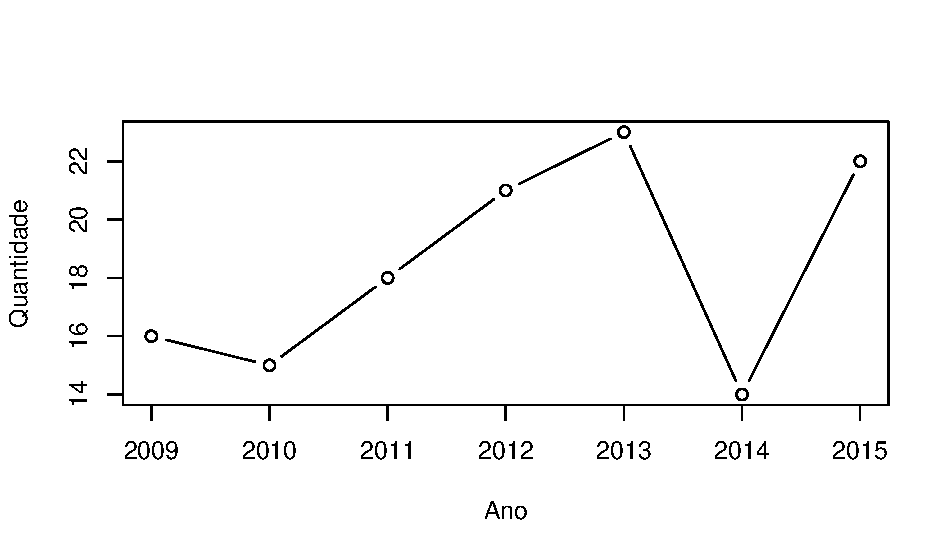
\includegraphics[width=1\textwidth]{./imagens/im_tools.pdf}
    \caption{Quantidade de soluções submetidas ao OAEI}
        \footnotesize{Fonte: \cite{cheatham2015results}.}
        \label{fig:oaei_imtools}
\end{figure}

Porém, de acordo com \citeonline{homoceanu2014putting}, apesar dos bons resultados apresentados, as soluções não estão prontas para alinhar dados automaticamente de forma confiável. Para isso, foi realizado um experimento equivalente ao executado pela OAEI. Entretanto, utilizando dados reais, que foram obtidos de 5 fontes diferentes (Freebase\footnote{\url{http://www.freebase.com/}}, DBPedia\footnote{\url{http://dbpedia.org}} , LinkedMDB\footnote{\url{http://www.linkedmdb.org}}, DrugBase\footnote{\url{http://www.drugbase.de/de/}} e NewYork Times\footnote{\url{http://www.nytimes.com}}). Além disso, o experimento permitiu notar que as características do modelo não eram considerados durante o processo de correspondência de instâncias.
        
Dentre as propriedades com suporte inadequado,  destaca-se a propriedade owl:sameAs, que é responsável por identificar recursos equivalentes. Além disso, essa se trata de uma propriedade transitiva. Dessa forma, se existem dois recursos equivalentes R1 e R2 e existe um terceiro recurso R3 que é equivalente a R2, então R1 é equivalente a R3. Como representado na Figura \ref{sameAs}.Tais características fazem com que a propriedade owl:sameAs seja uma das  mais utilizadas para alinhar dados na Web. Dessa forma, utilizar ferramentas que levem em consideração as características das propriedades é de grande importância para alinhar dados de forma confiável.
\begin{figure}[h]
\centering
\begin{tikzpicture}[node distance=1cm, auto,]
 %nodes
 \node[ellipse,draw] (r3) {R3};
 
 \node[above=of r3] (dummy) {};
 \node[right= of dummy,ellipse,draw](r2) {R2}
        edge[pil,<->, bend left=45] node[auto] {owl:sameAs} (r3);
 
 \node[left= of dummy,ellipse,draw] (r1) {R1}
        edge[dashed,<->, bend right=45] node[auto] {owl:sameAs} (r3)
        edge[pil,<->, bend left=45] node[auto] {owl:sameAs} (r2);
\end{tikzpicture}
\caption{Transitividade da propriedade owl:sameAs}
\label{sameAs}
\end{figure}

Neste contexto, este trabalho propõe uma abordagem independente de contexto para o alinhamento de dados conectados por meio de um processo de alinhamento que leva em consideração aspectos dos dados e  características do modelo ontológico. Assim, os recursos/instâncias analisados, além de alinhados através das propriedades de dados, podem ser alinhados través seus relacionamentos. Ademais, a proposta trata o problema do alinhamento entre datasets reais, permitindo que seja possível alinhar datasets distribuídos na Web de forma confiável.

\section{Objetivo}

Essa abordagem visa disponibilizar um mecanismo útil que permita alinhar semiautomaticamente recursos entre datasets diferentes. Além disso, a proposta também pretende facilitar a identificação e alinhamento de recursos duplicados dentro do mesmo dataset.
Dessa forma, o trabalho lida com aspectos mais gerais, como facilitar o alinhamento de dados, quanto com problemas específicos, como a definição de métricas para a análise de similaridade entre recursos, que sejam capazes de suportar os problemas provenientes dos datasets reais. Apesar de ser um trabalho com enfoque em engenharia de software, as suas contribuições estão mais voltadas para a área de Dados Conectados. Segue algumas dessas contribuições:

\begin{itemize}
        \item Construção de um processo para alinhar dados conectados independente de contexto;
        \item Definição de uma função de similaridade que contempla problemas provenientes de datasets reais (acentuação, ausência de propriedades, formatação e outros);
\end{itemize}

\section{Estrutura do trabalho}

Esta dissertação está dividida em 7 capítulos. O Capítulo 1 introduz a problemática e os objetivos do trabalho proposto, enaltecendo a necessidade de uma abordagem capaz de alinhar dados conectados. No Capítulo 2, são apresentados os conceitos relacionados ao tema deste trabalho, como RDF, Ontologias, Dados Conectados, Algoritmos de similaridade e Alinhamento de Dados Conectados.

No Capítulo 3, são apresentados os trabalhos relacionados à abordagem proposta. Algumas abordagens de alinhamento são descritas bem como comparadas com a solução proposta. Na conclusão do capítulo é apresentada uma tabela comparativa entre a abordagem proposta e os trabalhos relacionados apresentados.

O Capítulo 4 mostra como a proposta foi desenvolvida, tanto no processo de alinhamento por intermédio de um diagrama de atividades como na arquitetura através de um diagrama de componentes. Neste capítulo, todas as etapas do processo bem como os componentes da arquitetura são descritos detalhadamente.

No Capítulo 5 é apresentado um estudo de caso. Nele é descrita a plataforma QIE, um sistema que cruza dados da Revista Brasileira de Informática na Educação (RBIE), Simpósio Brasileiro de Informática na Educação (SBIE) e Workshop de informática na Escola (WIE) com dados extraídos da plataforma LATTES. Além disso, é descrito como o processo foi utilizado para alinhar os dados dos pesquisadores e de suas produções científicas entre essas bases.

No Capítulo 6, um experimento foi projetado para avaliar, em termos de eficácia através das métricas de precisão, revocação e medida-f, a abordagem proposta, em comparação com RiMOM \cite{zhang2015rimom} , Lily \cite{wang2015lily} e LogMap \cite{jimenez2015logmap}. Cada conjunto de alinhamento gerado é avaliado e uma discussão geral é apresentada ao final do capítulo.

Por fim, no Capítulo 7, são apresentadas as considerações finais deste trabalho. bem como são definidos alguns trabalhos futuros.

\chapter{Fundamentação e Trabalhos Relacionados}
\label{cap:fundamentacao}
Este capítulo está estruturado em duas seções, a primeira apresenta os conceitos necessários para o entendimento desse trabalho. A segunda apresenta os trabalhos que estão relacionados à correspondência de instância.

\section{Fundamentação Teórica}
O objetivo desta seção é apresentar a fundamentação teórica referente ao foco deste trabalho, fazendo uma pequena introdução  sobre conceitos da área que auxiliam na compreensão da pesquisa desenvolvida.

\subsection{RDF (Resource Description Framework)}

RDF trata-se de um \textit{framework} de descrição de recursos, trabalhando como um alicerce para a construção de Dados Conectados. Em concordância com tecnologias Web, bem como Dados Conectados, o modelo RDF utiliza URIs para identificação de recursos, permitindo que os recursos sejam descritos uniformemente na Web. Basicamente, o RDF é estruturado em triplas do tipo sujeito, predicado, objeto (ver Figura \ref{fig:spo}). 

\begin{figure}[!ht]
	\centering
	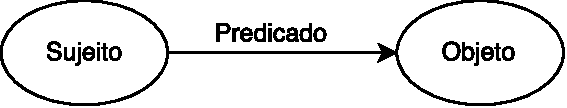
\includegraphics[width=0.5\textwidth]{./imagens/Sujeito-predicado-objeto.pdf}
    \caption{Estrutura da tripla RDF}
%	\footnotesize{Fonte: Próprio autor.}
	\label{fig:spo}
\end{figure}

A estrutura do RDF pode se materializar de várias formas. Cada uma dessas formas recebe o nome de serialização RDF. Atualmente existe um conjunto considerável de serializações tais como: RDF/XML, Turtle, N-Triples e outros. Onde cada serialização tem um uso em potencial. Por exemplo, Turtle é usado para ser lido por humanos, pois ele é melhor estruturado para isso. 

Vale a pena salientar que RDF é um framework de descrição, não sendo responsável por atribuir semântica aos recursos descritos, sendo as ontologias responsáveis por esta função. Por esta razão, um número considerável de processos de publicação de Dados Conectados \cite{bizer2007publish, hyland2011joy, villazon2011methodological, Avila2015} recomenda o reuso de ontologias. 

\subsection{Ontologias}
Os Dados Conectados fazem uso de ontologias como suporte formal para representação de conhecimento, pois só RDF não é o bastante para que máquinas consigam entender a relação entre os dados. Desta forma, as ontologias têm um papel fundamental na modelagem e descrição de dados. A palavra ontologia vem do Grego \textit{ontos} e \textit{logos}, significando conhecimento do ser. Em filosofia, ontologia refere-se ao estudo do ser. Em Computação, de maneira informal, uma ontologia define um conjunto de conceitos e suas relações, tais como a terminologia (vocabulário do domínio), definição explícita dos conceitos essenciais, suas classificações, taxonomias, relações e axiomas do domínio, incluindo hierarquias e restrições \cite{deved2006semantic}. Em 1993, \citeauthor{gruber1993translation} definiu ontologia como uma especificação explícita de uma conceitualização. Em 1997, \citeauthor{borstw1997construction} definiu ontologia como uma especificação formal de uma conceitualização compartilhada. Em 1998, \citeauthor{studer1998knowledge} unificaram as duas definições, desta forma ontologia pode ser definida como uma especificação formal e explícita de uma conceitualização compartilhada. Para melhor entendimento, abaixo seguem detalhes sobre os termos citados nessa definição: 
% * <profsean@gmail.com> 2017-01-18T19:49:08.414Z:
% 
% > \citeauthor{studer1998knowledge}
% Aqui o formato da citação está errado... Não entendi o motivo...
% 
% ^ <armandobs14@gmail.com> 2017-01-18T20:06:42.666Z:
%
% Isso ocorre por erro no bibtex, estou ajustando.
%
% ^ <armandobs14@gmail.com> 2017-01-18T20:06:50.399Z.
\begin{itemize}
	\item \textbf{Explícita:} definições de conceitos, relações, restrições e axiomas; 
	\item \textbf{Formal:} compreensível para agentes e sistemas; 
	\item \textbf{Conceitualização:} modelo abstrato de uma área de conhecimento; 
	\item \textbf{Compartilhada:} conhecimento consensual. 
\end{itemize}
Pode-se concluir, a partir das características supracitadas sobre ontologias, que o conhecimento é explícito. Esse conhecimento equivale à descrição de determinada área do conhecimento, garantindo um conhecimento “consensual” sobre tal área. A partir do momento em que há um consenso, há a possibilidade e a viabilidade de compartilhar tais ontologias e integrá-las a outras áreas de conhecimento (através de outras ontologias).

\subsection{Dados Conectados}
O termo Dados Conectados (do inglês Linked Data) é a tradução oficial para o conceito na língua portuguesa \cite{Isotani2015}. Segundo o W3C, Dados Conectados pode ser entendido como o núcleo da Web Semântica, tendo como objetivo prover a integração e raciocínio de dados disponíveis na Web. Além disso, \citeonline{berners2006linked} ressalta que Dados Conectados não se trata apenas de pôr dados na internet, mas fazer conexões entre eles, permitindo que pessoas ou máquinas possam explorar a Web dos dados.

Para conectar os dados disponíveis na Web com qualidade, foram desenvolvidas as boas práticas. Essas boas práticas são fundamentadas em tecnologias Web como ressaltam \citeonline{Isotani2015}. Além dessas tecnologias, vale a pena destacar os quatro princípios básicos de Dados Conectados \cite{berners2006linked}: 

\begin{enumerate}
	\item Usar URI para a identificação de recursos
	\item Usar HTTP URIs para que seja possível buscar pelos recursos 
	\item Prover informação útil para as URIs consultadas através de padrões (RDF e SPARQL) 
	\item Incluir links para outras URIs. Possibilitando a descoberta de novos recursos
\end{enumerate}

É possível dividir os princípios em duas categorias. A primeira categoria é composta pelos dois primeiros princípios, estando relacionada a identificação e resolução desses recursos através de URI e HTTP URIs. A segunda categoria está relacionada de forma prática à conexão dos dados, utilizando RDF para especificar como os recursos são descritos e URIs que apontam para outros recursos, conectando de fato os dados.

\subsection{Algoritmos de similaridade}

Algoritmos de similaridade podem ser entendidos como funções utilizadas para medir a semelhança entre objetos. Essas funções podem ser utilizadas em diferentes contextos, partindo de correções ortográficas até tarefas de processamento de linguagem natural (PLN). A escolha de uma abordagem pode variar de acordo com o contexto de aplicação. Além disso, existe mais de uma abordagem dentro do mesmo contexto. A Figura \ref{fig:tecnicas_similaridade} apresenta uma visão geral sobre as abordagens de acordo com seu contexto de aplicação. 

\begin{figure}[!ht]
	\centering
	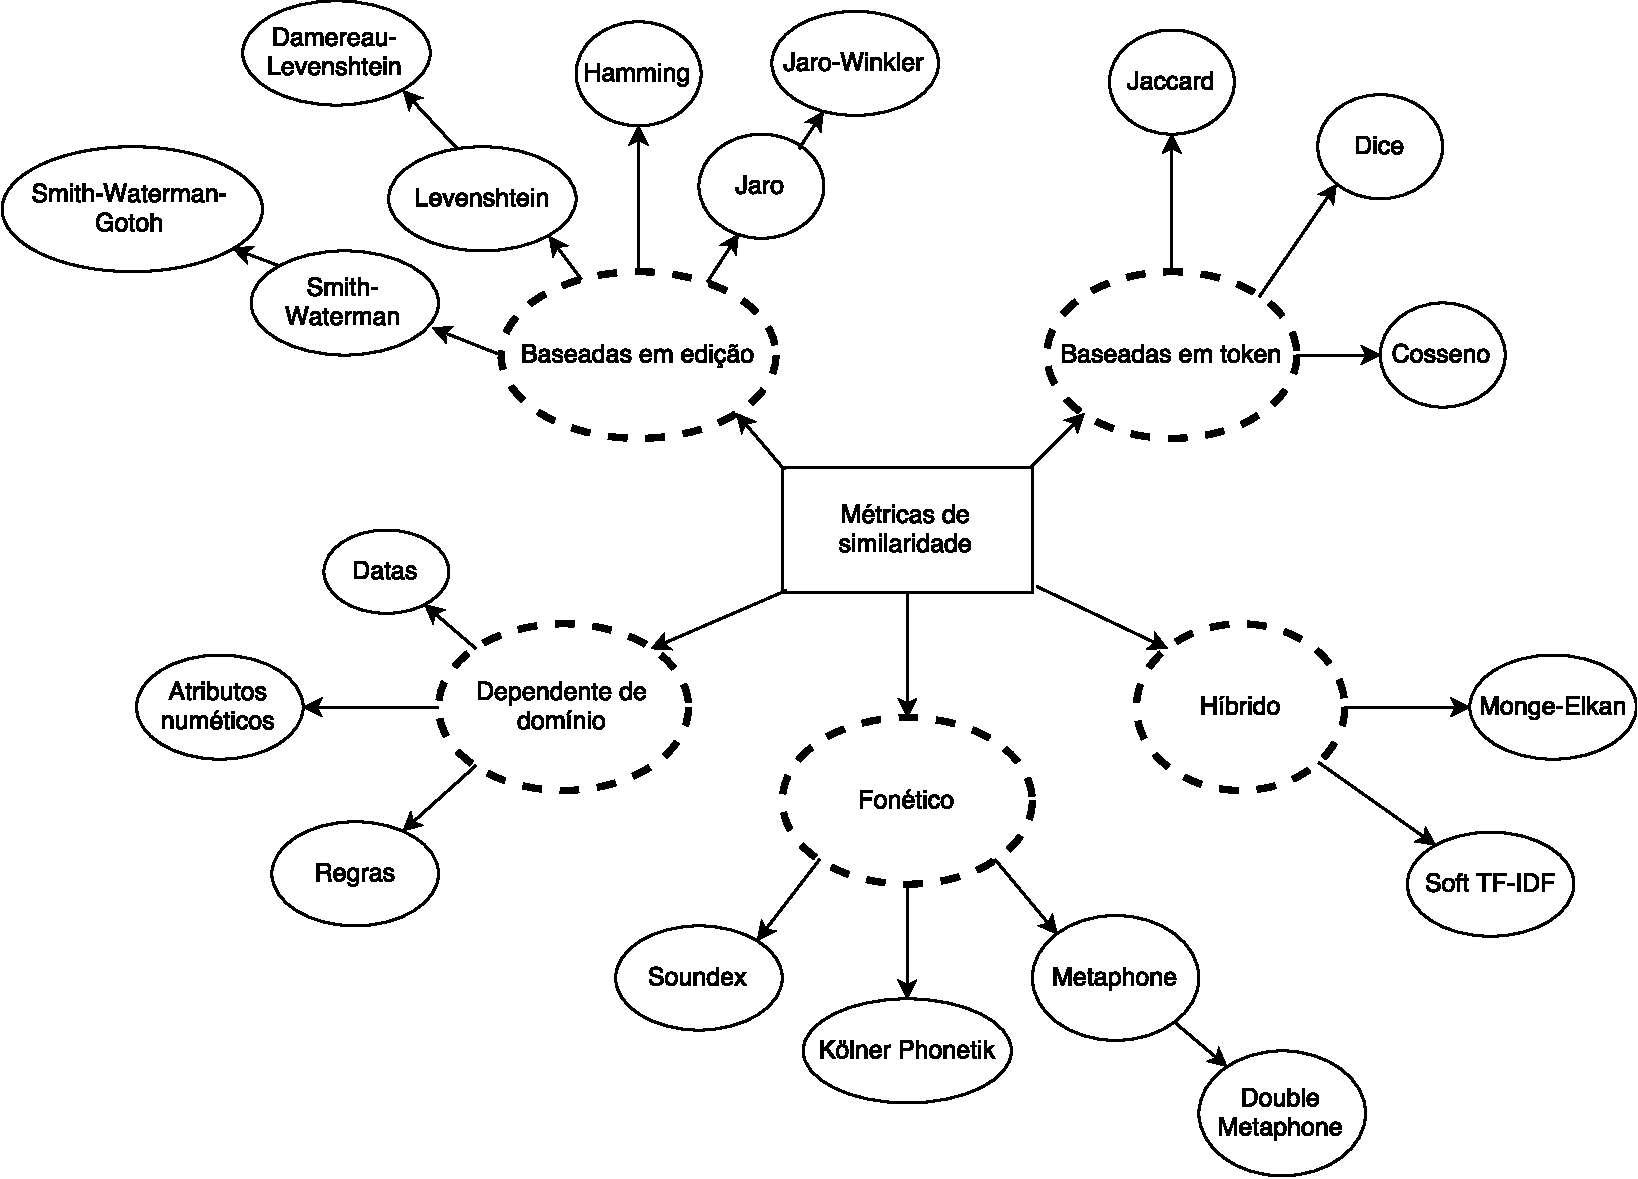
\includegraphics[width=1\textwidth]{./imagens/similarity-metrics.pdf}
	\caption{Visão geral das tecnicas de similaridade}
	\label{fig:tecnicas_similaridade}
\end{figure}

%descrever as categorias pontilhadas 

%No contexto de similaridade entre palavras por exemplo, um dos algoritmos de similaridade mais conhecidos pela comunidade foi proposto por Levenshtein em 1965 \cite{levenshtein1966binary}, que se baseia na quantidade mínima de edições (remoções e adições) necessárias para que uma palavra seja igual a outra.

%Dependendo do objeto a ser analisado (palavras, textos e objetos complexos) existem diferentes abordagens (baseadas em caractere, baseadas em \textit{token}) \cite{cohen2003comparison}. Abordagens baseadas em caractere (e.g. Levenshtein) realizam a comparação letra por letra. Já as abordagens baseadas em \textit{tokens} (e.g. Jaro) consideram a palavra como um corpo único.

Nesta proposta, foi utilizada uma generalização do algoritmo de Monge-Elkan \cite{monge1996field}, que tem o objetivo de dar um peso maior a \textit{tokens} mais semelhantes. Inicialmente, Monge-Elkan foi desenvolvido com o objetivo de calcular a semelhança entre textos que possuem vários \textit{tokens}, onde a similaridade de cada \textit{token} é calculada através da média das similaridades internas, que é provida por uma técnica baseada em caractere (e.g. Cosseno, Jaro, Dice). Essa abordagem se destaca em cenários de desordem ou ausência de \textit{tokens}. Além disso, esse algoritmo explora os benefícios providos pelas abordagens baseadas caractere (e.g. erros de digitação, erros de OCR e erros ortográficos) \cite{jimenez2009generalized}.

\subsection{Alinhamento de Dados Conectados}

Alinhar Dados Conectados  trata-se de um processo que tem como objetivo identificar e mesclar recursos que representam a mesma entidade do mundo real. Segundo \citeonline{homoceanu2014putting}, no contexto de dados conectados temos a seguinte definição para o problema:

\begin{equation}
f\left( { URI }_{ i },{ URI }_{ j } \right) :=\begin{cases} \mbox{verdadeiro, se } sim\left( { URI }_{ i },{ URI }_{ j } \right) >\theta  \\ \mbox{falso, caso contrário} \end{cases}\mbox{com }{ URI }_{ i } \in { D }_{ i }\mbox{ e }{ URI }_{ j } \in { D }_{ j }
\end{equation}

onde 1 $\leq$ i,j $\leq$ n, e $sim()$ é uma função que é capaz de calcular a similaridade entre os recursos e $\theta$ é o parâmetro que regula o nível de qualidade para o alinhamento, que também pode ser conhecido como limiar ou \textit{threshold}. Além disso, é possível ressaltar outros benefícios que surgem a partir da conexão entre dados, sendo elas: 

\begin{itemize}
	\item \textbf{Integração semântica de dados:} Refere-se ao melhoramento das técnicas existentes para descobertas de mapeamento (semi) automático entre ontologias heterogêneas e distribuídas; 
	\item \textbf{Reconhecimento de identidade:} Refere-se à capacidade de identificar se descritores de recursos distintos estão relacionados à mesma entidade do mundo real; 
	\item\textbf{ População de ontologias:} Refere-se à descoberta de relacionamentos entre novas instâncias e as instâncias já existentes na base de conhecimento. 
\end{itemize}

Segundo \citeonline{ferrara2008towards}, para que uma abordagem seja capaz de identificar recursos que identifiquem a mesma entidade do mundo real com propriedade essa deve satisfazer diferentes requisitos, que estão  dispostos em três categorias (ver Figura \ref{fig:imrequirements}).

\begin{figure}[!ht]
	\centering
%	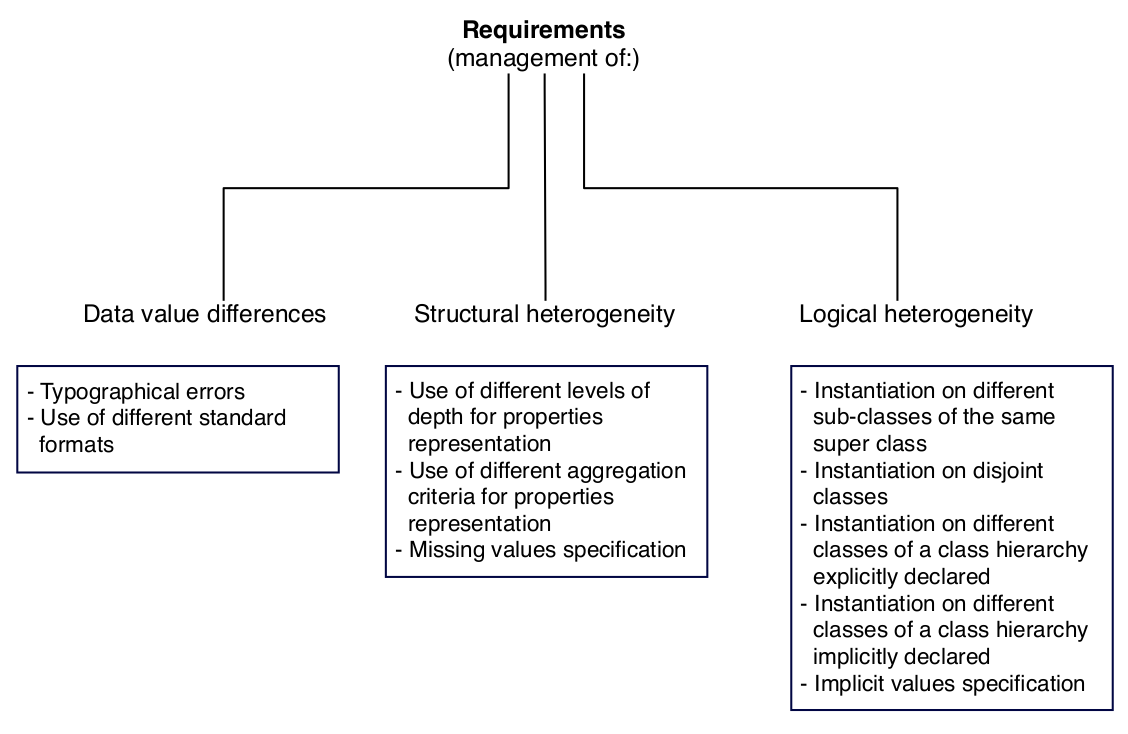
\includegraphics[width=0.9\textwidth]{./imagens/IMRequirements.png}
	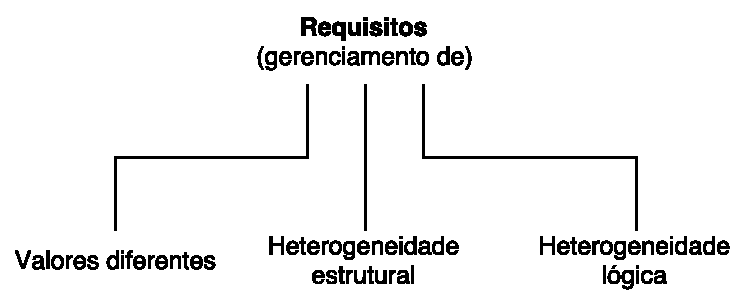
\includegraphics[width=0.9\textwidth]{./imagens/im_requirements.pdf}
    \caption{Requisitos para soluções de alinhamento de dados}
	\footnotesize{Fonte: baseado em \cite{ferrara2008towards}}
	\label{fig:imrequirements}
\end{figure}

\textbf{Valores diferentes:}
% * <profsean@gmail.com> 2017-01-18T20:15:13.295Z:
% 
% > Diferença de Valores:
% "Diferença de valores" (como está no texto) ou "Valores diferentes" (como está na figura)?
% 
% ^ <armandobs14@gmail.com> 2017-01-18T20:17:47.903Z:
%
% Ajustei para deixar de acordo com a imagem.
%
% ^ <armandobs14@gmail.com> 2017-01-18T20:17:50.727Z.
Um algoritmo de correspondência de instância deve reconhecer valores correspondentes, sempre que possível, mesmo quando esses valores possuem erros. Para mitigar esse problema, a comunidade utiliza abordagens como algoritmos de similaridade e transformação de valores.


\textbf{Heterogeneidade Estrutural:}
Instâncias que pertencem a ontologias diferentes diferem não somente entre propriedades e valores, mas também na sua estrutura. Desta forma, algoritmos de alinhamento de dados devem identificar propriedades semelhantes em ambos os recursos.


\textbf{Heterogeneidade Lógica:}
% * <profsean@gmail.com> 2017-01-18T20:18:47.062Z:
% 
% > Heterogeneidade Lógica:
% Não explicou...
% 
% ^ <armandobs14@gmail.com> 2017-01-18T20:36:14.777Z:
%
% O autor não descreve o que seria de fato a heterogeneidade lógica, dessa forma descrevi de acordo o meu entendimento.
%
% ^ <armandobs14@gmail.com> 2017-01-18T20:36:21.108Z.
A heterogeneidade lógica trata-se de um problema de alinhamento de ontologias, o qual não é levado em consideração no processo de alinhamento de dados, no entanto, faz-se necessário em tarefas de inferência. Esse problema diz respeito à semântica atribuída aos termos, havendo situações em que o mesmo termo pode ter significados diferentes atribuídos a ele (\textit{e.g.} manga - fruta e manga - vestimenta).

Diante do exposto, a comunidade vem desenvolvendo alternativas para a identificação de correspondência de instâncias. Diante disso, a seção a seguir apresenta os trabalhos relacionados a esta proposta.
% * <armandobs14@gmail.com> 2017-01-18T21:47:58.426Z:
% 
% > Diante do exposto, a comunidade vem desenvolvendo alternativas para a aperfeiçoar as soluções para a correspondência de instâncias . Diante disso, a seção aseguir apresenta trabalhos relacionado a esta proposta.
% 
% Melhorar a conexão entre os parágrafos.
% 
% ^ <armandobs14@gmail.com> 2017-01-19T01:07:55.371Z.

\section{Trabalhos Relacionados}
% * <profsean@gmail.com> 2017-01-18T20:19:34.451Z:
% 
% > Trabalhos
% Independente de juntar ou não os capítulos, é importante encadear esta parte do texto com a anterior... Ficou uma quebra... muda completamente de assunto...
% 
% ^ <armandobs14@gmail.com> 2017-01-19T01:08:23.836Z:
%
% Adicionei um parágrado ao final do capítulo anterior.
%
% ^ <armandobs14@gmail.com> 2017-01-19T01:08:25.949Z.
\label{cap:relacionados}
Neste capítulo serão apresentadas duas ferramentas para o alinhamento de dados conectados. As ferramentas apresentadas a seguir foram selecionadas  devido ao seu destaque na edição de 2016 do relatório publicado pela Ontology Alignment Evaluation Initiative (OAEI), mais especificamente na trilha referente à correspondência de instâncias (\textit{Instance Matching}). Inicialmente, a OAEI avaliava apenas ferramentas de alinhamento de ontologias, dando início à avaliação de soluções para alinhar dados em 2009. Desde então, um número crescente aplicações vêm sendo submetidas \cite{cheatham2015results}.
% * <profsean@gmail.com> 2017-01-18T20:22:17.708Z:
% 
% > Desde então, um número crescente aplicações vêm sendo submetidas
% Dados que comprovem? Evidências disto?
% 
% ^ <armandobs14@gmail.com> 2017-01-18T20:46:12.594Z:
%
% Citei o mesmo paper que utilizei na introdução.
%
% ^ <armandobs14@gmail.com> 2017-01-19T01:08:32.597Z.
% * <profsean@gmail.com> 2017-01-18T20:21:19.611Z:
% 
% > devido ao seu destaque
% Deveria explicar melhor que destaque foi esse... Preocupa o fato de ter considerado apenas 2 (e a escolha não estar bem clara)... também não sei se outras ferramentas com características mais próximas não deveriam ter sido consideradas (baseadas em instâncias)...
% 
% ^ <armandobs14@gmail.com> 2017-01-18T20:51:26.403Z:
%
% Citei que dentro do OAEI, essas ferramentas foram submetidas para a track de instance matching.
%
% ^ <armandobs14@gmail.com> 2017-01-19T01:10:08.818Z.

\subsection{AgreementMakerLight (AML)}
Desenvolvido em parceria entre o Instituto Gulbenkian de Ciência, a Universidade de Lisboa, e a Universidade de Illinois, o AgreementMakerLight é uma ferramenta de alinhamento de ontologias. De acordo com \cite{fariaoaei}, o AML se baseia inicialmente em técnicas e similaridade léxica, tendo como ênfase o uso de fontes externas como \textit{background}.

O AML conta com três algoritmos para alinhamento voltados a correspondência de instâncias, sendo eles o \textit{HybridStringMatcher}, o \textit{ValueStringMatcher} e o \textit{Value2LexiconMatcher}. O primeiro utiliza diversas abordagens para gerar a similaridade, sendo elas a comparação entre frases, palavras. Além disso, essa abordagem hibrida também explora a \textit{WordNet}. O segundo utiliza o mapeamento de valor para gerar calcular a similaridade, penalizando pares nos quais anotações ou propriedades de dados não são os mesmos. Por fim, o terceiro une as duas abordagens anteriores.

Apesar do AML possuir diferentes algoritmos de alinhamento na ferramenta, todos eles trabalham apenas no nível dos dados. Consequentemente, as características das propriedades são desconsideradas ao longo do processo de correspondência.

\subsection{RiMOM-2016}
Baseando-se no RiMOM  \cite{li2009rimom}, \citeonline{zhang2016rimom} desenvolveram o RiMOM-2016, que é uma ferramenta para alinhar dados conectados. Ela implementa um número considerável de abordagens para alinhar, cuja escolha é realizada através dos metadados extraídos da ontologia. Além disso, o RiMOM-2016 utiliza um índice invertido para indexar os objetos e consequentemente gerar pares candidatos para um possível alinhamento. A geração dos pares é realizada quando dois recursos compartilham pelo menos um predicado e objeto.

\begin{figure}[!ht]
	\centering
	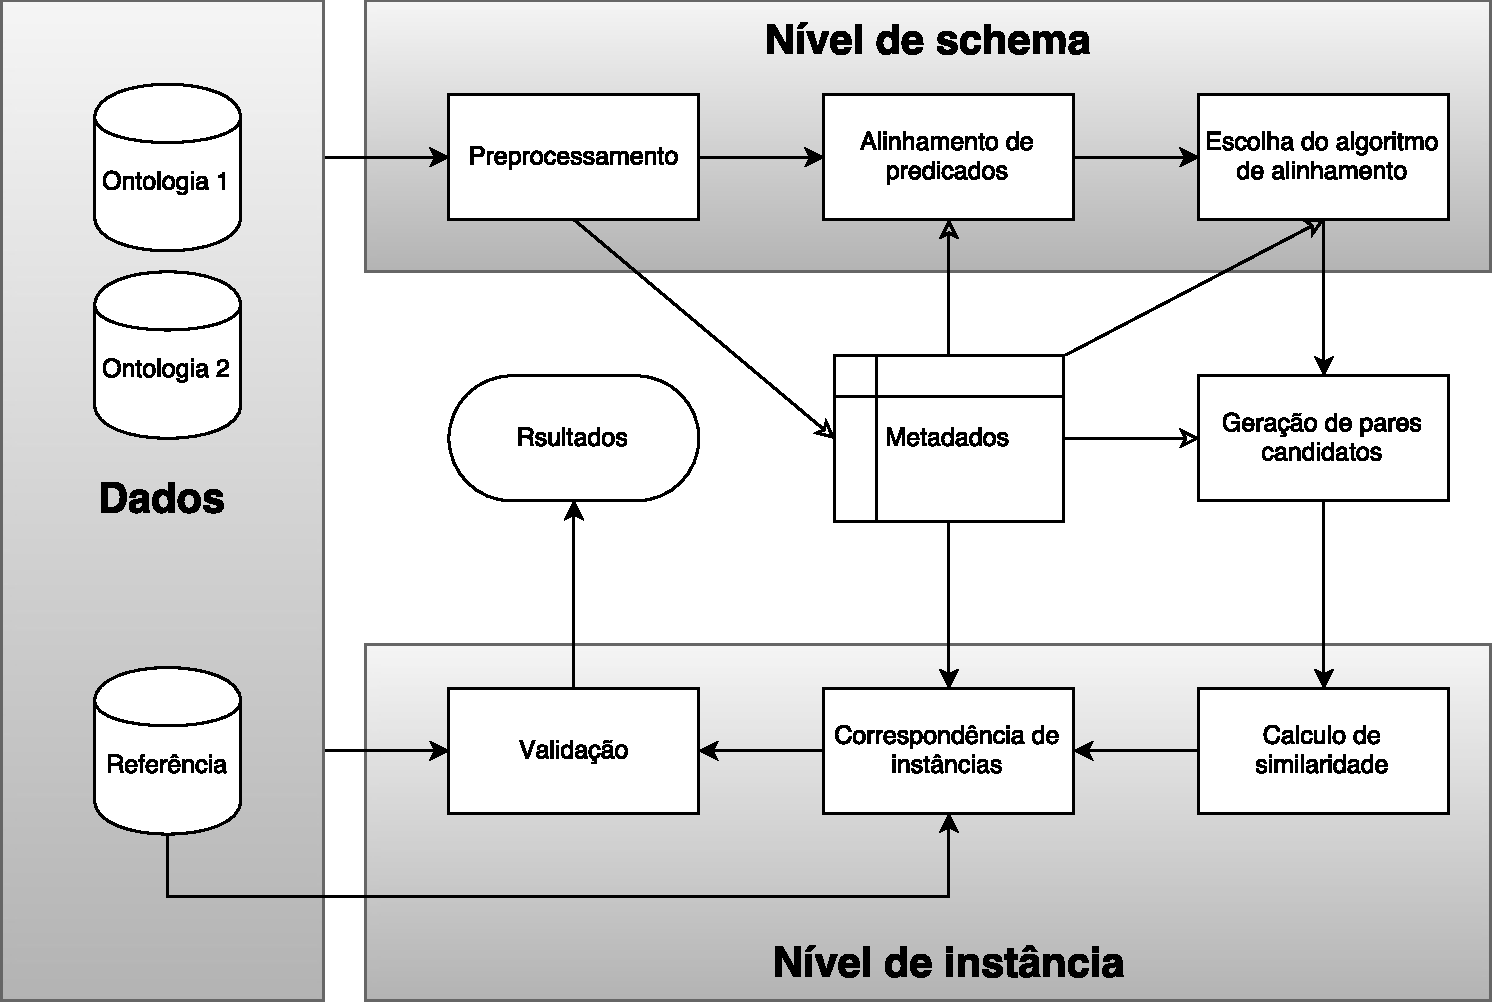
\includegraphics[width=0.8\textwidth]{./imagens/rimom_2016.pdf}
    \caption{Arquitetura do RiMOM-2016}
	\footnotesize{Fonte: adaptado de \cite{zhang2016rimom}}
	\label{fig:rimom}
\end{figure}

Por um lado, o índice invertido permite que um número menor de comparações seja realizado. Por outro lado, a etapa de construção desse índice não considera que os objetos indexados podem conter qualquer tipo de erro. Além disso, como pode ser visto na Figura \ref{fig:rimom}, o RiMOM-2016 utiliza as ontologias apenas para alinhar as propriedades e como entrada para a geração de metadados.

\subsection{Comparação com a proposta}

Neste capítulo, algumas das principais ferramentas existentes foram apresentadas. Essas ferramentas tem o objetivo de alinhar dados conectados através de diversas abordagens. Dentre os sistemas apresentados, nenhum deles contempla o alinhamento de dados como foco principal, sendo variações de ferramentas existentes para o alinhamento de ontologias.
% * <profsean@gmail.com> 2017-01-18T20:34:14.738Z:
% 
% > nenhum deles contempla o alinhamento de dados como foco principal
% Não tem nenhuma? Será que vc pesquisou direito? Será que não deveria ter buscado ferramentas que fazem alinhamento baseado em instâncias? Se não me engano o pessoal do Marco Antonio Casanova, prof. da PUC-Rio estava trabalhando com isso... não sei se deixaram ferramentas disponíveis. Sugiro dar uma pesquisada porque o Bernardo (que estará na sua banca) foi aluno do Casanova...
% 
% ^ <armandobs14@gmail.com> 2017-01-18T20:44:36.267Z:
%
% Nesse caso, quis dizer que nenhuma das ferramentas apresentadas tem o alinhamento de dados como foco principal, pois são adaptações de soluções para o alinhamento de ontologias.
%
% ^ <armandobs14@gmail.com> 2017-01-19T01:11:11.956Z.

Esta seção tem o objetivo de apresentar um comparativo entre os trabalhos relacionados e o presente estudo. Para isso, consideramos os seguintes critérios: 
\begin{enumerate}
\item \textbf{Quantidade de \textit{datasets} suportados:} Este critério refere-se à quantidade de de \textit{datasets} que podem ser utilizados para no processo de correspondência de instâncias. Normalmente, apenas dois \textit{datasets} são suportados simultaneamente. Com isso, a troca de um dos \textit{datasets} é necessária.
\item \textbf{Tipo de suporte à ontologia:} Este critério refere-se à maneira como as ontologias são exploradas pela ferramenta de correspondência de instâncias, podendo ser classificada como dirigida ou baseada em ontologia.  Uma ferramenta pode ser classificada como dirigida por ontologia quando explora a modelagem conceitual com o objetivo de escolher o conjunto de atividades que são utilizados no processo. Por outro lado, uma ferramenta é dita baseada em ontologias quando a modelagem conceitual é a base para o processo de correspondência.
\item \textbf{Utilização de computação específica:} Este critério refere-se à utilização de algoritmos específicos para os \textit{datasets} que serão utilizados no processo de correspondência de instâncias com o objetivo de melhorar a precisão das correspondências estabelecidas.
\item \textbf{Exploração dos conceitos presentes na ontologia:} Este critério refere-se a exploração dos conceitos presentes na modelagem conceitual. Além disso, as características dos relacionamentos são consideradas (\textit{e.g.} transividade).
\end{enumerate}

\begin{table}[h]
	\centering
	\caption{Comparação entre os trabalhos}
	\label{tab:comparacao}
	\begin{tabular}{@{}llll}
		\toprule
		\textbf{Critérios de comparação}                    & \textbf{RiMOM} & \textbf{AML} & \textbf{Proposta} \\ \midrule
		(1) Quantidade de \textit{datasets} suportados    & 2              & 2            & 2+                \\
% * <profsean@gmail.com> 2017-01-18T20:40:50.085Z:
% 
% > Quantidade de \textit{datasets} suportados
% Por que os dois só consideram 2 datasets? Você quer dizer no alinhamento consideram 2 a 2 entidades?
% 
% ^ <armandobs14@gmail.com> 2017-01-18T20:55:00.624Z:
% 
% Eles são capazes de realizar a correspondência de dois datasets por vez (e.g. Lattes <-> SBIE). Dessa forma, para utilizar um outro dataset é necessário trocar um deles (e.g. Lattes <-> WIE). Já a proposta suporta mais de dois datasets por vez (e.g. Lattes <-> [SBIE,WIE,SBIE]).
% 
% ^ <armandobs14@gmail.com> 2017-01-19T01:11:59.559Z.
		(2) Tipo de suporte à ontologia                     & Dirigido       & Dirigido     & Baseado           \\
% * <profsean@gmail.com> 2017-01-18T20:40:17.651Z:
% 
% > Tipo de suporte
% Isto deveria ter sido melhor explicado... o que quer dizer? O que é dirigido e baseado?
% 
% ^ <armandobs14@gmail.com> 2017-01-19T01:12:16.222Z.
		(3) Utilização de computação específica             & Sim            & Sim          & Não               \\
		(4) Exploração dos conceitos presentes na ontologia & Não            & Não          & Sim               \\ \bottomrule
	\end{tabular}
\end{table}

Contudo, apesar das ferramentas se mostrarem capazes de encontrar correspondência entre instâncias, ainda deixam a desejar em alguns critérios, tais como a utilização de computação específica para os \textit{datasets}, além da pouca exploração das ontologia, que são utilizadas apenas para a geração de metadados, com o objetivo de escolher entre as abordagens de correspondência disponíveis. Diferentemente das ferramentas citadas, a proposta utiliza ontologias para guiar o processo de correspondência de instância. Além disso, essa abordagem permite que o usuário defina como o alinhamento deve ser realizado.

Outro diferencial da proposta em relação aos trabalhos relacionados está no que chamamos de alinhamento em cascata, que consiste na utilização de instâncias que pertencem a conceitos relacionados ao conceito cujas instâncias serão alinhadas.  O alinhamento em cascata vai além das instâncias, ele explora os relacionamentos existentes. A partir disso, é possível encontrar novas correspondências. Ademais, a proposta permite que as correspondências entre as instâncias sejam armazenadas diretamente na base de triplas (\textit{triple store}) em que estão armazenadas.
% * <profsean@gmail.com> 2017-01-18T20:43:43.697Z:
% 
% > alinhamento em cascata, que consiste na utilização de instâncias que pertencem a conceitos relacionados ao conceito cujas instâncias serão alinhadas.
% Isto deveria ser melhor explicado... Por que o alinhamento em cascata é importante? Como esta importância é percebida?
% 
% ^ <armandobs14@gmail.com> 2017-01-19T01:54:05.765Z.
%\chapter{Trabalhos Relacionados}

Neste capítulo serão apresentadas três soluções (RiMOM-2015, LogMap e Lily) para o alinhamento de dados conectados. As ferramentas apresentadas a seguir foram selecionadas devido ao seu destaque na edição de 2015 do relatório publicado pela Ontology Alignment Evaluation Initiative (OAEI). Inicialmente, a OAEI avaliava apenas ferramentas de alinhamento de ontologias, dando início à avaliação de soluções para alinhar dados apenas em 2009. Desde então, um número crescente aplicações vêm sendo submetidas.

\section*{RiMOM-2015}
Baseando-se no RiMOM \cite{li2009rimom}, \citeonline{zhang2015rimom} desenvolveram o RiMOM-2015, que é uma ferramenta para alinhar dados conectados. Ela implementa um número considerável de abordagens para alinhar, cuja escolha é realizada através dos metadados extraídos da ontologia. Além disso, o RiMOM-2015 utiliza um índice invertido para indexar os objetos e consequentemente gerar pares candidatos para um possível alinhamento. A geração dos pares é realizada quando dois recursos compartilham pelo menos um predicado e objeto.

Por um lado, o índice invertido permite que um número menor de comparações seja realizado. Por outro lado, a etapa de 
construção desse índice não considera que os objetos indexados podem conter qualquer tipo de erro. Além disso, como pode ser visto na Figura \ref{fig:rimom}, o RiMOM-2015 utiliza as ontologias apenas para alinhar as propriedades e como entrada para a geração de metadados.

\begin{figure}[!ht]
	\centering
	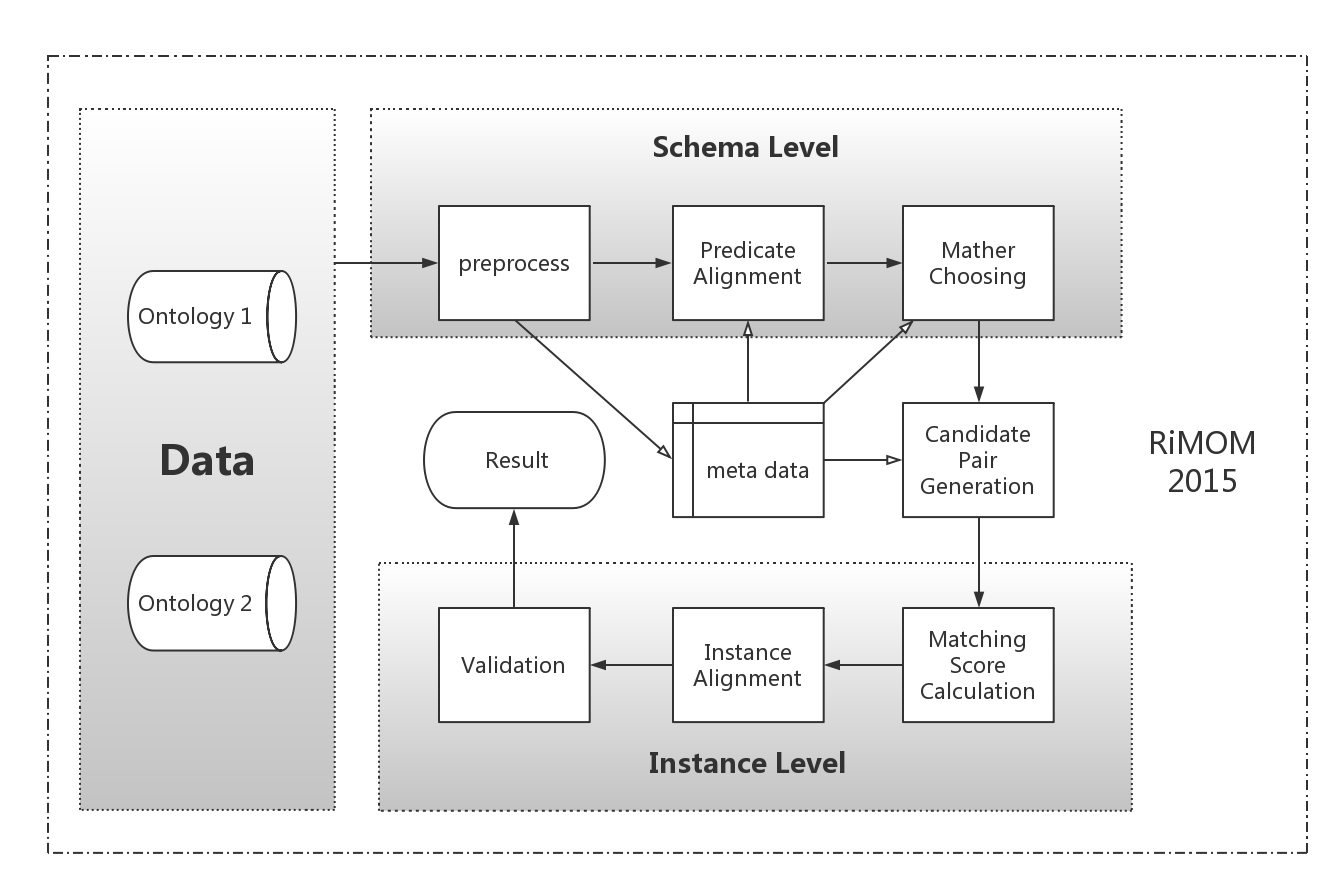
\includegraphics[width=0.8\textwidth]{./imagens/RiMOM_2015.png}
    \caption{Arquitetura do RiMOM-2015}
%	\footnotesize{Fonte: \cite{ferrara2008towards}2008towards}}
	\label{fig:rimom}
\end{figure}

\section*{LogMap}
Segundo \citeonline{jimenez2011logmap}, LogMap é uma solução para o alinhamento de ontologias. Logo, para dar suporte ao alinhamento de dados algumas alterações foram realizadas \cite{jimenez2015logmap}. Dentre as adaptações aplicadas está a adição de algoritmos de similaridade de texto.

o LogMap também utiliza índice invertido durante o processo de alinhamento. No entanto, o índice é gerado a partir das labels e de variações extraídas do WordNet ou do Unified Medical Language System (UMLS), com pode ser visto na Figura \ref{fig:logmap}. Além disso, raciocinadores como Hermit e Condor são utilizados para melhorar os resultados da indexação. 
Atualmente, existem três variações do LogMap, sendo elas LogMapC, LogMapBio e LogMapLt.  No primeiro, foi adicionado princípios de consistência e localidade. Essa variação foi desenvolvida com o objetivo de elevar a precisão dos alinhamentos apesar do decrescimento do recall. No segundo, foi utilizada uma extensão para o BioPortal, utilizando-o como um repositório de ontologias, permitindo que ontologias sejam recuperadas em tempo de execução. Por fim, mas não menos importante, se trata de uma versão “lightweight” do LogMap onde foi adicionado técnicas de similaridade de texto.

\begin{figure}[!ht]
	\centering
	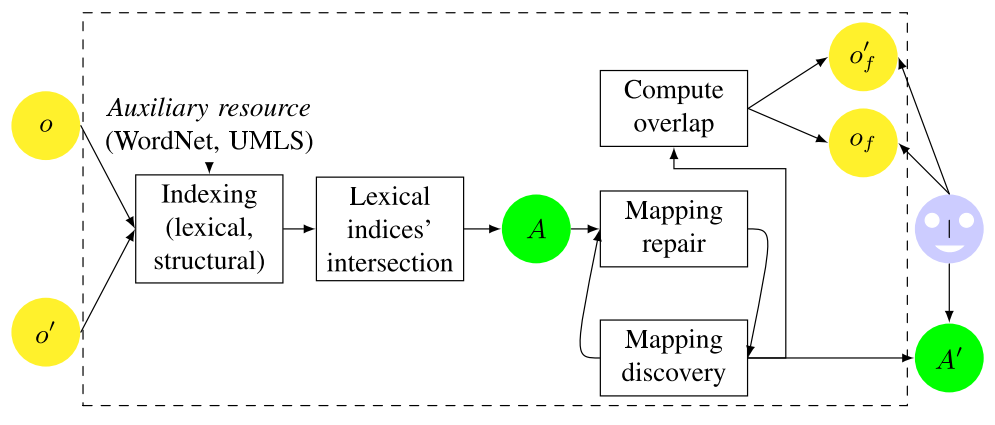
\includegraphics[width=0.8\textwidth]{./imagens/logmap.png}
    \caption{Arquitetura do LogMap}
	\footnotesize{Fonte: \cite{euzenat2013d}}
	\label{fig:logmap}
\end{figure}

\section*{Lily}
Desenvolvida durante o doutorado na Southeast University localizada em Nanjing no ano de 2008. Segundo \citeonline{wang2015lily}, Lily se trata de uma solução para o alinhamento de ontologias. Ela é composta por 5 estratégias principais, das quais apenas uma se dedica ao alinhamento de dados.
o Lily processo de alinhamento utilizado é composto pelo pré processamento, alinhamento e pós processamento (Figura \ref{fig:lily}).  A primeira etapa, consiste em analisar as ontologias de entrada para gerar metadados que serão utilizados para determinar parâmetros e estratégias. Na segunda, a ferramenta calcula a similaridade entre elementos de ontologias diferentes. Por fim, a etapa de pós processamento é responsável por exportar e refinar os alinhamentos gerados.

\begin{figure}[!ht]
	\centering
	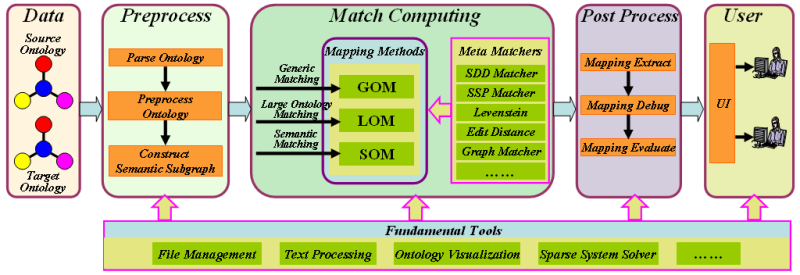
\includegraphics[width=0.9\textwidth]{./imagens/lily.png}
    \caption{Arquitetura do Lily}
	\footnotesize{Fonte: \cite{euzenat2013d}}
	\label{fig:lily}
\end{figure}

\section*{Comparação com a proposta}

Neste capítulo, algumas das principais ferramentas existentes foram apresentadas. Estas ferramentas tem o objetivo de alinhar dados conectados através através de diversas abordagens.
Dentro os sistemas apresentados, nenhum deles têm o alinhamento de dados como foco principal. Além disso, as abordagens apresentadas estão não permitem integração com soluções de armazenamento de triplas (Virtuoso, OWLim e outros), o que inviabiliza o seu uso em soluções mais complexas. Por fim, é descrito que as ferramentas são baseada em soluções de alinhamento de ontologias, porém a exploração no processo de alinhamento se limita à geração de metadados para auxiliar na escolha da estratégia que deve ser tomada. A tabela \ref{tab:comparacao} sumariza e compara os trabalhos relacionados com a proposta.

\begin{table}[h]
\centering
\caption{Comparação entre os trabalhos}
\label{tab:comparacao}
\begin{tabular}{@{}cccc@{}}
\toprule
Ferramenta & Integração a tripleStor & Suporte à ontologia & Foco               \\ \midrule
RiMOM-2015 &                         & X                   & Ontologia + Dados \\
LogMap     &                         & X                   & Ontologia + Dados \\
Lily       &                         & X                   & Ontologia + Dados \\
Proposta   & X                       & X                   & Dados             \\ \midrule
\end{tabular}
\end{table}

\chapter{Processo de alinhamento}
\label{cap:processo}
Neste capítulo, será apresentado o processo proposto para alinhar dados. Como exibido na Figura \ref{fig:processo}, o processo é composto por 4 etapas principais, sendo elas: selecionar \textit{datasets}, identificar conceitos, listar recursos e alinhar dados. cada etapa do processo será descrita nas subseções a seguir.

\begin{figure}[!h]
	\centering
	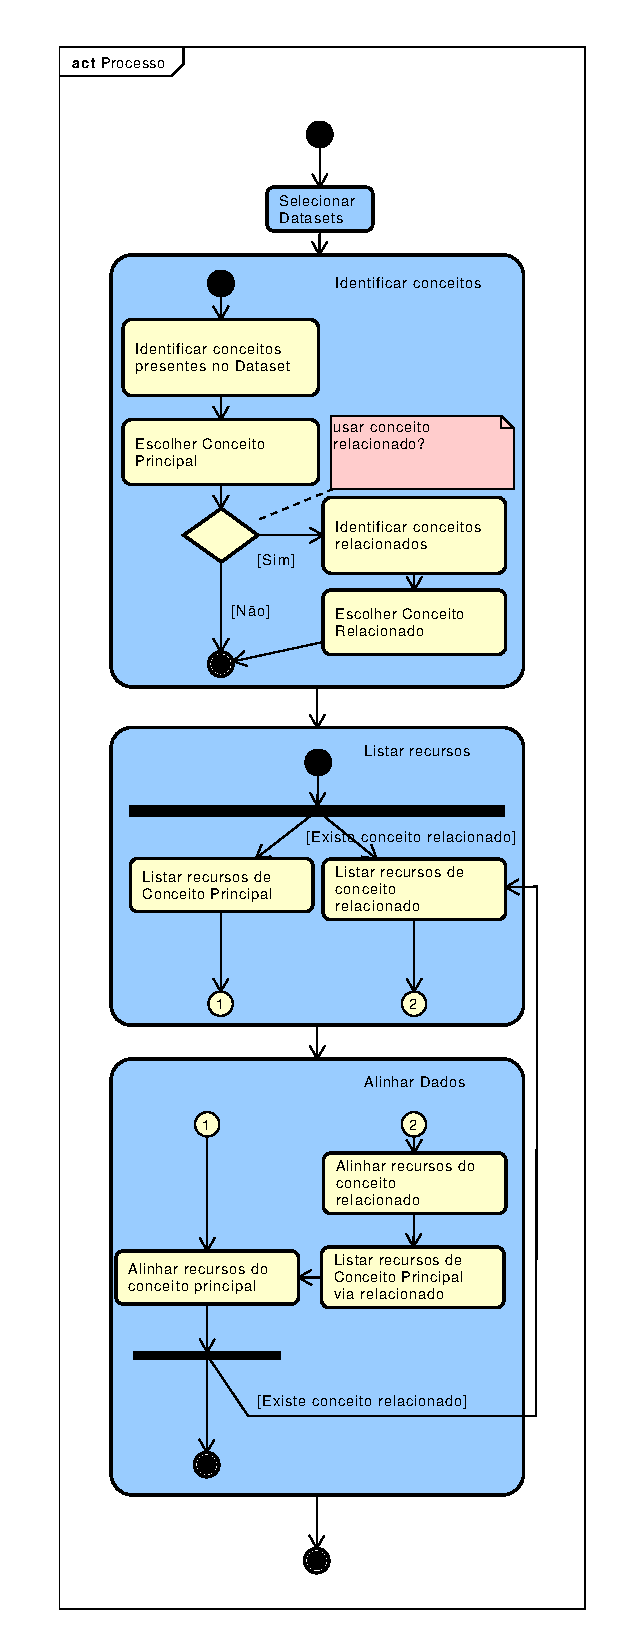
\includegraphics[width=0.55\textwidth]{./imagens/processo.pdf}
    \caption{Processo de alinhamento de dados conectados}
	\label{fig:processo}
\end{figure}

\section{I - Selecionar Datasets}
A etapa de selecionar \textit{datasets} trata da determinação de quais conjuntos de dados serão alinhados. A seleção de um \textit{dataset} está sujeita a alguns critérios, tais como: estar estruturado em triplas e utilizar conceitos modelados em ontologias/vocabulários. Tais critérios foram determinados de acordo com o escopo do processo, pois este está limitado à dados conectados. Além de se adequar ao escopo, os critérios cumprem os requisitos mínimos para a execução do processo.
Complementarmente, a comunidade já disponibiliza ferramentas e processos para a publicação de dados conectados na Web, o que não é o foco desse processo. Além disso, é importante destacar que ao modelar os dados em qualquer processo de publicação de dados conectados são utilizadas ontologias/vocabulários que podem servir como base.

\section{II - Identificar Conceitos}
\label{sec:prop_identificar}
Para auxiliar na escolha do conceito bem como os conceitos que estão relacionados foi desenvolvida duas consultas SPARQL. A primeira consulta explora a ontologia, principalmente as relações rdfs:domain e rdfs:range dos  as propriedades de objeto (ver código \ref{lst:sparql}). A segunda explora os dados e as relações estabelecidas pelas instâncias.
Na consulta \ref{lst:sparql}, a linha 4 tem o papel de recuperar todos os conceitos pertencentes na ontologia ou vocabulário. Na linha 5 é aplicada uma restrição. Nesta os conceitos devem ser domínio ou range de uma relação. Consequentemente, uma instância desse conceito será sujeito ou objeto de uma tripla (ver Figura \ref{fig:subgrafo1}).
\begin{figure}[!h]
	\centering
	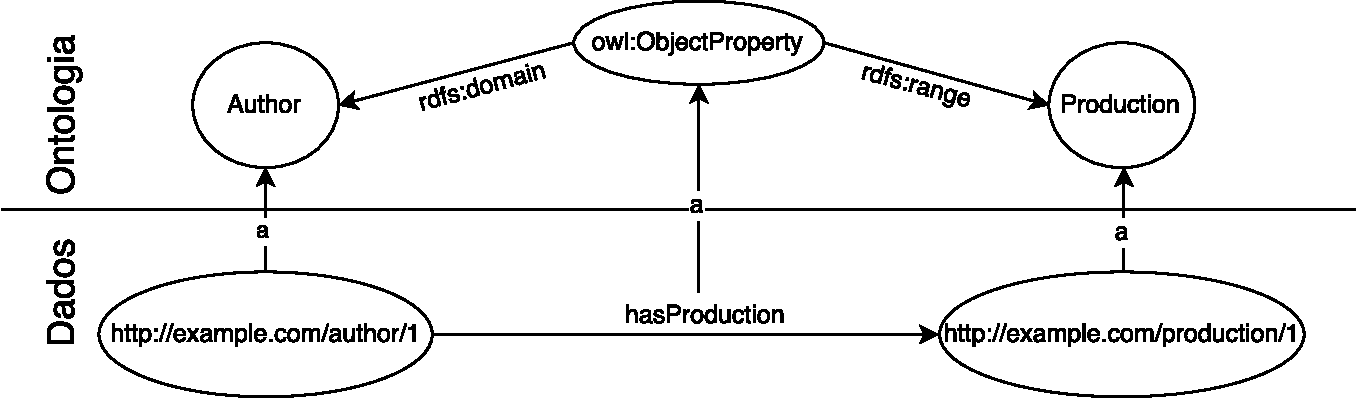
\includegraphics[width=0.9\textwidth]{./imagens/subgrafo_semantico.pdf}
	\caption{Relação entre ontologia e dados}
	\label{fig:subgrafo1}
\end{figure}

\begin{lstlisting}[captionpos=b, caption= Consulta SPARQL para identificação de conceito, label=lst:sparql,
basicstyle=\ttfamily,frame=single]
PREFIX rdf: <http://www.w3.org/1999/02/22-rdf-syntax-ns#>
PREFIX rdfs: <http://www.w3.org/2000/01/rdf-schema#>
select distinct ?Concept count(*) as ?count where {
[] 	a ?Concept.
?Concept 	(^rdfs:domain|^rdfs:range) ?o.
}
group 	by ?Concept	
order 	by desc(?count)
\end{lstlisting}

A consulta \ref{lst:sparql2} é comporta de duas partes, visto que o conceito pode modelar instâncias que são sujeito ou objeto de uma relação. Na primeira parte, o conceito selecionado representa o sujeito da tripla. Através das relações das instâncias é possível recuperar os conceitos que modelam as instâncias  relacionadas (objetos). Na segunda parte ocorre o inverso, o conceito representa o objeto da tripla e os conceitos que representam os sujeitos são recuperados.

\begin{lstlisting}[captionpos=b, caption=Query SPARQL para recuperação de conceitos relacionados, label=lst:sparql2,
   basicstyle=\ttfamily,frame=single]
PREFIX rdf: <http://www.w3.org/1999/02/22-rdf-syntax-ns#>
PREFIX rdfs: <http://www.w3.org/2000/01/rdf-schema#>


select distinct ?type where {
	values ?Concept{<URI do conceito escolhido>}
	{
		?instance rdf:type ?Concept; ?p ?o.
		?p rdf:type owl:ObjectProperty.
		?o rdf:type ?type.
	}
	union
	{
		?s ?p ?o.
		?p rdf:type owl:ObjectProperty.
		?o rdf:type ?Concept.
		?s rdf:type ?type.
	}
}

\end{lstlisting}

Como resultado do Código \ref{lst:sparql2} é provida uma lista contendo os conceitos relacionados ao conceito escolhido. Neste momento, o usuário deve escolher, quais conceitos relacionados ele deseja utilizar para melhorar o alinhamento do conceito escolhido. A escolha dos conceitos, assim como a quantidade de conceitos relacionados pode ser realizada de forma arbitrária. Essa decisão influenciará tanto no tempo que o processo levará para concluir, quanto na quantidade de recursos alinhados ao final do processo, pois para cada conceito relacionado haverá uma nova execução das etapas (iii) e (iv). Esse loop é necessário, pois alguns alinhamentos serão possíveis apenas através da relação entre esses conceitos.

\section{III - Listar recursos}
A etapa de listar recursos pode ser entendida como a recuperação dos recursos que pertencem aos conceitos. É importante destacar que a listagem/recuperação de recursos da base de conhecimento pode ser executada mais de uma vez durante o processo, gerando um conjunto de recursos para cada conceito escolhido. Além disso, essa etapa é responsável pela geração de pares candidatos, onde os recursos do \textit{Dataset} $D_{1}$ são comparados com os recursos do \textit{dataset} $D_{2}$.


\section{IV - Alinhar Dados}
A etapa de alinhamento de dados está dividida em duas atividades sendo elas: (i) alinhamento simples e (ii) alinhamento em , que serão detalhadas nas subseções a seguir.

\subsection{alinhamento simples}
\label{im_simples}
Para alinhar os recursos é necessário executar alguns procedimentos, sendo eles o tratamento dos dados, comparação entre recursos e análise da similaridade. O primeiro procedimento se refere a transformações nas propriedades dos recursos. Essas transformações são necessárias para auxiliar os algoritmos de similaridade a analisar melhor a semelhança entre os recursos. No procedimento de comparação, cada uma da propriedades são analisadas. Caso uma propriedade não pertença a um dos recursos, ela é dispensada da comparação. A Figura  \ref{fig:resources} apresenta a comparação entre as propriedades de cada recurso.

\begin{figure}[!h]
	\centering
	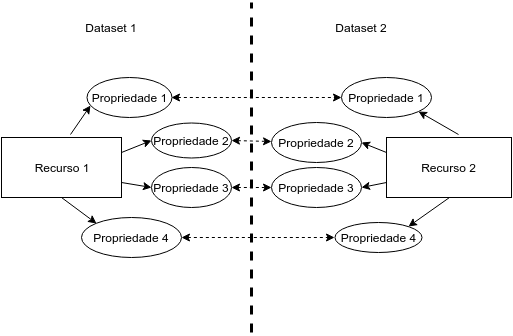
\includegraphics[width=0.6\textwidth]{./imagens/resources.png}
    \caption{Comparação entre recursos}
	\label{fig:resources}
\end{figure}

Para definir a similaridade entre as instâncias foram usadas duas equações. A Equação \ref{eq:properties_definition} define o conjunto de propriedades que será considerado durante a comparação entre os recursos, que será obtido a partir da diferença entre  o maior conjunto de propriedades e o conjunto de propriedades que deve ser desconsiderado. Logo:

\begin{equation}
P_f =M a x  ( P_{r1} ,P_{r2} ) - P_d
\label{eq:properties_definition}
\end{equation}

Onde:
\begin{itemize}
	\item $P_{r1}$ – Propriedades do recurso 1;
	\item $P_{r2}$ –  Propriedades do recurso 2;
	\item $P_d$ –  Propriedades que devem ser desconsideradas;
	\item $M a x  ( P_{r1} ,P_{r2} )$ – Retorna o maior conjunto de propriedades;
\end{itemize}

A Equação \ref{eq:similaridade} trata da função de similaridade entre recursos, essa equação pode ser entendida como a média das similaridades entre dois recursos.

\begin{equation}
SR  = \frac{1}{|P_f|} { \sum_{i = 1}^{P_f} {S(V(R_1,P_f[i]);V(R_2,P_f[i]))}}
\label{eq:similaridade}
\end{equation}

Onde:

\begin{itemize}
	\item S – Função de similaridade léxica;
	\item V(R,P) – Valor da propriedade P em um recurso R;
	\item $R_1$ – Recurso 1;
	\item $R_2$ – Recurso 2;
\end{itemize}

O valor gerado pelo componente de similaridade é enviado para o componente de alinhamento.

\subsection{Alinhamento em cascata}
\label{sub:cascata}
O alinhamento em cascata recebe esse nome devido as atividades que são executadas nesta etapa que são: Alinhamento simples dos recursos relacionados, Recuperação das instâncias que pertencem ao conceito principal que estão relacionadas aos recursos relacionados e alinhamento simples das instâncias recuperadas.

%\begin{figure}[!h]
%	\centering
%	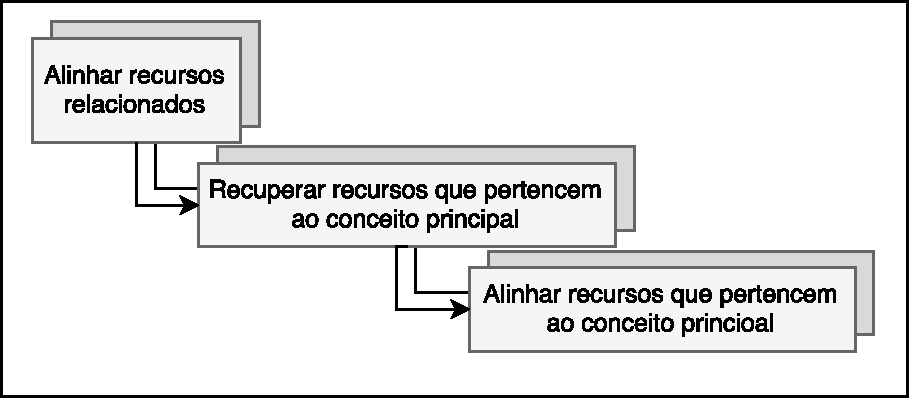
\includegraphics[width=0.6\textwidth]{./imagens/cascata.pdf}
%	\caption{Alinhamento em cascata}
%	\label{fig:cascata}
%\end{figure}

\subsubsection{Alinhar Recursos}

Nesta atividade as instâncias que pertencem aos conceitos selecionados são alinhados. Para alinhar esses recursos é executado a etapa de alinhamento simples.

\subsubsection{Recuperar Recursos do conceito principal}
\label{recuperao}

A recuperação das instâncias que pertencem ao conceito principal é realizada a partir do  alinhamento dos recursos relacionados.A Figura \ref{fig:relacionados} representa abstratamente a construção dos pares candidatos a partir dos alinhamentos dos recursos relacionados.

\subsubsection{Alinhar Recursos Recuperados}

A partir das listas de candidatos geradas na atividade \ref{recuperao} o processo de alinhamento simples é executado.

\begin{figure}[!ht]
	\centering
	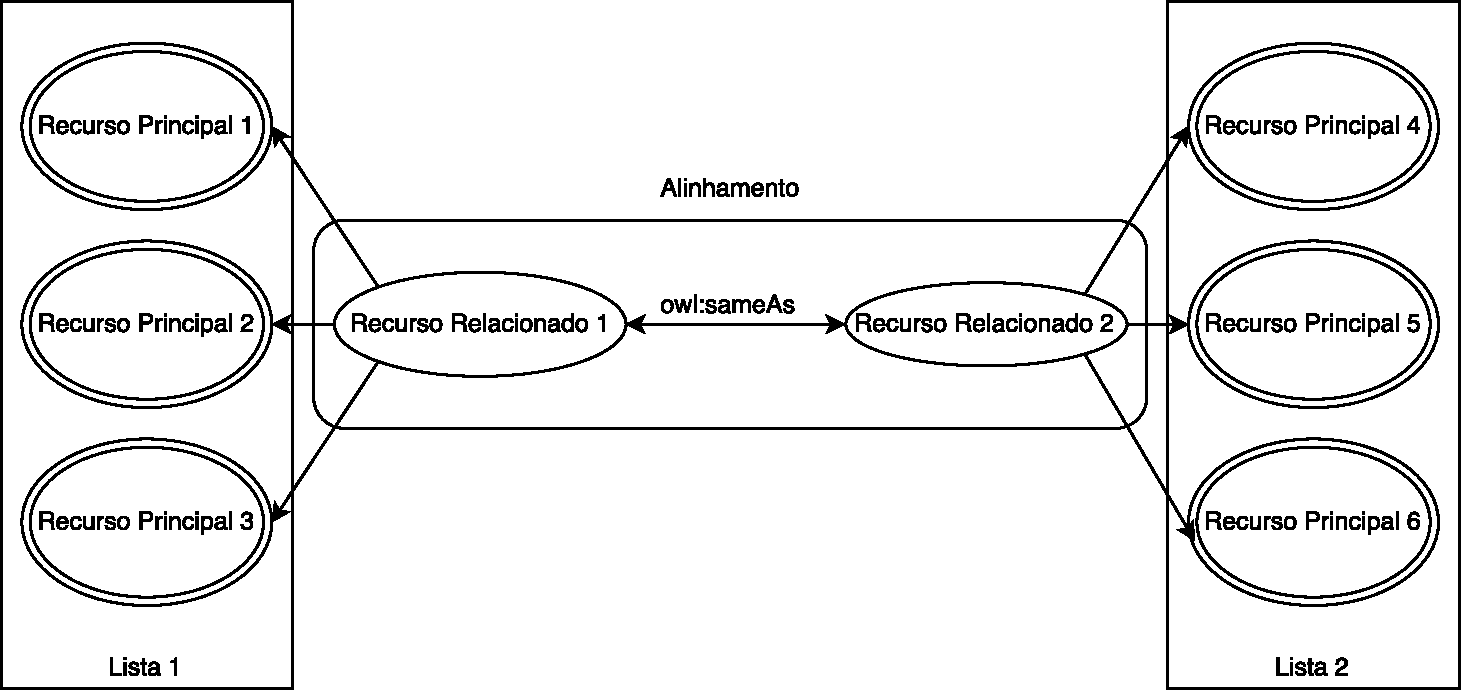
\includegraphics[width=0.8\textwidth]{./imagens/relacionados.pdf}
    \caption{Construção de pares candidatos a partir de recursos relacionados}
	\label{fig:relacionados}
\end{figure}
\chapter{Implementação do Processo}
\label{cap:componentes}
A execução do processo ocorre por meio de componentes para a análise de similaridade, persistência dos dados, geração do alinhamento, lógica entre as etapas e pré-processamento (ver Figura \ref{fig:componentes}). Alguns componentes foram reusados, como o de similaridade léxica, que contém vários algoritmos para detectar a similaridade entre textos. Outros componentes foram desenvolvidos, como os responsáveis pela detecção da similaridade de recurso, alinhamento e outros.

\begin{figure}[!ht]
	\centering
	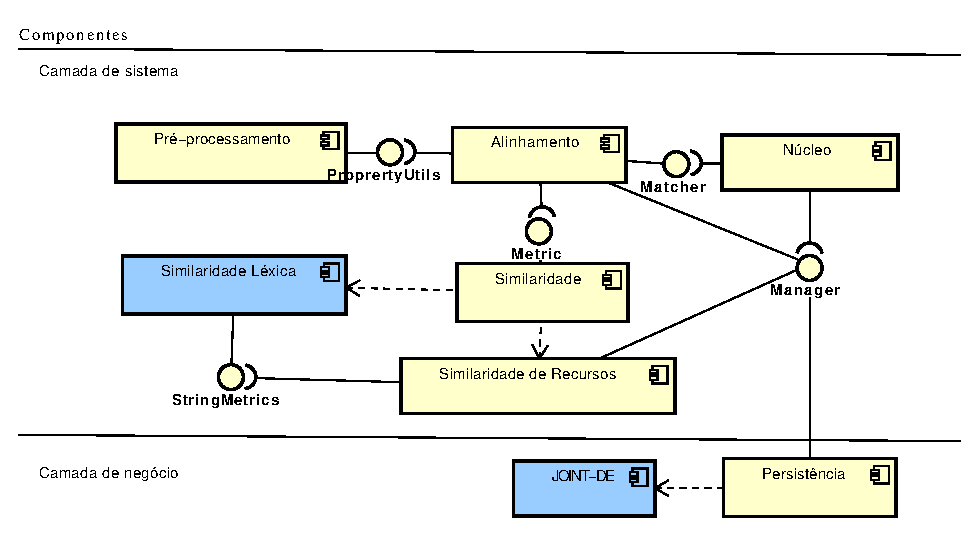
\includegraphics[width=1\textwidth]{./imagens/componentes.pdf}
    \caption{Componentes utilizados na implementação do processo}
	\label{fig:componentes}
\end{figure}

Apesar de existirem diversas soluções que contém algoritmos para o cálculo de similaridade e alinhamento entre recursos, optou-se pelo desenvolvimento de uma abordagem que contemplasse problemas provenientes de bases de dados reais (acentuação, ausência de propriedades, formatação e outros) \cite{castano2011ontology,ferrara2008towards}.
Os principais componentes utilizados são:

\section{Persistência}

O componente de persistência é responsável materializar as correspondências encontras pelo componente de alinhamento. Para isso, é utilizado o JOINT, que de acordo com \citeonline{holanda2013joint}, é um arcabouço para facilitar o desenvolvimento de aplicações baseadas em ontologia. As \textit{features} apresentadas pela ferramenta JOINT permitem que operações sejam realizada diretamente no servidor de triplas (Virtuoso, OWLim etc.). Além disso, essa ferramenta também suporta a execução de consultas SPARQL, que através de um sistema de tradução, transforma as triplas em objetos da linguagem Java.

A Figura \ref{fig:joint} apresenta a arquitetura do JOINT.

\begin{figure}[!ht]
	\centering
	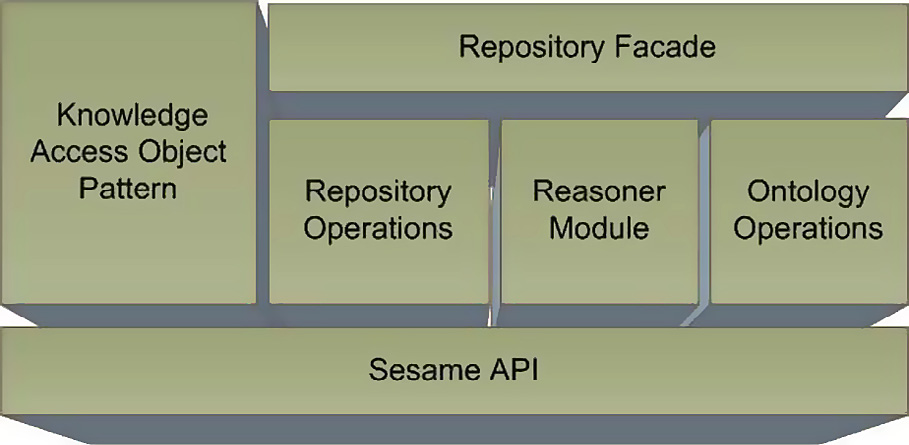
\includegraphics[width=1\textwidth]{./imagens/joint.png}
	\caption{Arquitetura da ferramenta JOINT}
	\footnotesize{Fonte: \cite{holanda2013joint}.}
	\label{fig:joint}
\end{figure}

\section{Similaridade}
O componente de similaridade é dividido em dois subcomponentes, sendo eles o de similaridade léxica e recurso. O primeiro utiliza métricas que analisam a similaridade entre palavras e textos. Algumas dessas técnicas são Levenshtein \cite{levenshtein1966binary}, Cosseno \cite{singhal2001modern}, Jaro-Winkler \cite{winkler1990string} e outros. O segundo componente, que se refere à similaridade de recurso, utiliza o primeiro e tem como função gerar a similaridade entre recursos.

Para o cálculo da similaridade dos recursos foi utilizada uma abordagem baseada na técnica de subgrafo semântico \cite{wang2008lily}. Na prática, um subgrafo semântico diz respeito às triplas que estão relacionadas a um recurso qualquer, que estão de acordo com a modelagem ontológica. A Figura \ref{fig:subgrafo} representa um subgrafo que relaciona um autor e sua publicação. Além de propriedades de objetos, um subgrafo também possui propriedades de dados, tanto do recurso principal (Author), quanto dos conceitos relacionados (Production). % O trecho de código \ref{lst:similaridade} descreve a implementação do cálculo de similaridade.

\begin{figure}[!ht]
	\centering
	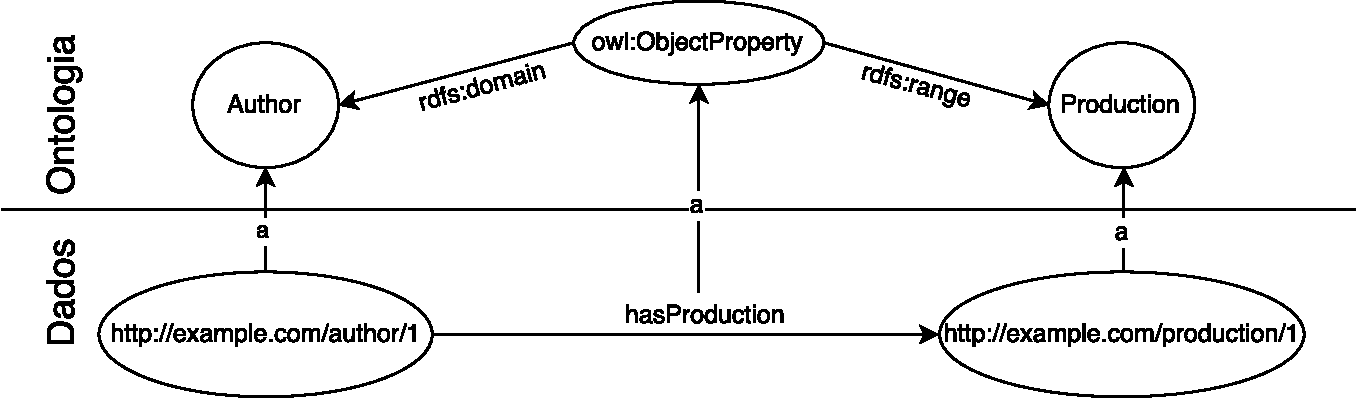
\includegraphics[width=0.9\textwidth]{./imagens/subgrafo_semantico.pdf}
    \caption{subgrafo que relaciona os conceitos Author e Publication}
	\label{fig:subgrafo}
\end{figure}

% \begin{lstlisting}[captionpos=b, caption= Trecho de código java para calcular a similaridade entre recursos, label=lst:similaridade,
%    basicstyle=\ttfamily,frame=single]
% float avg_similarity = 0;
% try {
%   //Gerando subgrafos
%   JSONObject graphA = resource1;
%   JSONObject graphB = resource2;

%   // Recuperando subgrafo com mais propriedades
%   if (graphA.length() > graphB.length()) {
%     JSONObject aux = graphA;
%     graphA = graphB;
%     graphB = aux;
%   }

%   // Numero de comparacoes internas
%   float innerComparisions = 0;

%   // Valor de similaridade para cada propriedade
%   float innerSimilaritySum = 0;

%   // Chaves de iteracao
%   Iterator keys = graphB.keys();

%   while (keys.hasNext()) {

%     //Recupera chave
%     String key = (String) keys.next();

%     // desconsiderando chaves que estiverem no set
%     if (propertySet != null && propertySet.contains(key)) continue;
%     try {

%       // Recuperando o valor da propriedade
%       Object pA = graphA.get(key);
%       Object pB = graphB.get(key);

%       // Casting para string
%       String propertyA = (pA instanceof JSONArray) ? ((JSONArray) pA).getString(0) : graphA.getString(key);
%       String propertyB = (pB instanceof JSONArray) ? ((JSONArray) pB).getString(0) : graphB.getString(key);

%       // Recuperando quantidade de tokens
%       int tokensizeA = propertyA.toString().split(" ").length;
%       int tokensizeB = propertyB.toString().split(" ").length;

%       //Similaridade temporaria
%       float tempSimirity = 0f;

%       // Recuperando Estrategia baseada na quantidade maxima de tokens
%       StringMetric metric1 = (StringMetric) MongeElkanMetricStrategy.getMetric(Math.max(tokensizeA, tokensizeB));

%       // Dispensando o tipo e a uri do recurso
%       if (key.equals("type") ||
%         key.equals("@id")) {
%         continue;

%         // Se for recurso
%     } else if (levels > 0 && propertyA.toLowerCase().contains("http://") && propertyB.toLowerCase().contains("http://")) {
%       innerComparisions++;
%       tempSimirity = this.compare(propertyA, propertyB, levels);

%       // Se for dado
%     } else {
%       innerComparisions++;
%       tempSimirity = metric1.compare(PropertyUtils.nameCleaning(propertyA, true), PropertyUtils.nameCleaning(propertyB, true));
%     }
%     System.out.println(key+" = "+tempSimirity);

%     // Atribuindo peso a similaridade
%     innerSimilaritySum+= tempSimirity * weight.getOrDefault(key,1f);
%   } catch (Exception e) {
%     continue;
%   }
% }

% // Definindo similaridade de recurso
% avg_similarity = innerSimilaritySum / innerComparisions;

% \end{lstlisting}


O valor gerado pelo componente de similaridade é enviado para o componente de alinhamento.
\section{Alinhamento}
O componente de alinhamento tem como responsabilidade determinar, de acordo com os valores obtidos na etapa de similaridade, se os recursos analisados realmente dizem respeito à mesma entidade do mundo real. Para determinar se o alinhamento deve ser realizado, este componente faz uso de limiares de aceitação, que são determinados previamente. Por esse motivo, o processo de alinhamento não é uma tarefa automática, pois precisa que os valores sejam ajustados. Existem diversas formas de determinar o valor do limiar, que vão desde executar várias vezes e analisar o melhor custo/benefício entre precisão e revocação até utilizar técnicas que atualizam o valor do limiar dinamicamente.


\section{Núcleo}

O componente de núcleo é responsável por concentrar e coordenar as configurações durante a execução. Atualmente, o componente de núcleo conta com três modalidades para a correspondência entre instâncias, sendo elas o alinhamento simples, que é executado em todas as modalidades, podendo também ser executado de forma independente, como mencionado na subseção \ref{im_simples}. O alinhamento em cascata, que é executando quando é escolhido um conceito relacionado ao conceito cujas instâncias se deseja alinhar. O processo de execução do alinhamento em cascada pode ser encontrado na subseção \ref{sub:cascata}. Por fim, o alinhamento em multicascata, que ocorre quando mais de um conceito relacionado é escolhido. Vale ressaltar que esta variação se trata do alinhamento em cascata de vários conceitos relacionados, que pode ser executado em paralelo.

\section{Pré-processamento}
O componente de pré-processamento tem como função realizar tratamentos nos textos que serão aplicados à função de similaridade. Alguns exemplos de tratamento são: tratamento de acentos, pontuação e outros.


\chapter{Experimento}
\label{cap:experimento}
Sabendo que o presente trabalho visa desenvolver um processo de alinhamento de dados  e  independente de contexto consolidado em uma ferramenta que seja capaz de realizar a correspondência de instâncias, afim de melhorar a eficácia das soluções de correspondência de instâncias. Este capítulo está dividido em quatro seções que abordam (i) Design de Experimento; (ii) Execução do experimento; (iii) Análise dos resultados e (iv) Principais conclusões obtidas.

\section{Design de Experimento}
Nesta seção, será detalhado o planejamento do experimento que foi projetado para este trabalho. Dentro do planejamento, encontra-se a definição da questão de pesquisa e derivação de hipóteses, a seleção das variáveis dependentes e independentes, a identificação da unidade experimental e a seleção do modelo experimental que será utilizado.

\subsection{Situando o problema}
A avaliação de ferramentas de correspondência de instâncias utilizada \textit{datasets} e um alinhamento de referência. Como mencionado na subseção \ref{sub:contribuicao}, isso permite que os desenvolvedores utilizem computação específica para os \textit{datasets}. Com isso, retomamos o nosso problema:

\textbf{(Problema Geral)} Como identificar que duas instâncias dizem respeito à mesma entidade do mundo real?
Atualmente, estratégias baseadas em similaridade, aprendizagem, regras e contexto \cite{Castano2011} vêm sendo utilizadas para resolver o problema. Porém, segundo \citeonline{Homoceanu2014} essa ferramentas para correspondência de instância não estão pontos para alinhar dados automaticamente de forma confiável. 

Diante disso, nos deparamos com nosso problema específico: 

\textbf{(Problema Específico)} Como melhorar a eficácias das ferramentas para correspondência de instâncias?

\subsection{Objetivos da Investigação}
A pesquisa a ser realizada é de caráter experimental e tem como objetivo geral \textbf{avaliar a eficácia das ferramentas de correspondência de instâncias}. O intuito do experimento é \textbf{refutar} as hipóteses nulas definidas na subseção \ref{sub:hipoteses} indicando que a abordagem proposta, apesar de não conter computação específica para os \textit{datasets} é capaz de criar correspondências com eficácia.

Formalmente, o objetivo da nossa investigação pode ser definido como \textbf{analisar} ferramentas de correspondência de instâncias \textbf{com a intenção de}  compará-los \textbf{a respeito} de sua eficácia \textbf{no ponto de vista} de geração de correspondência entre instâncias \textbf{no contexto} alinhamento de dados entre \textit{datasets} \textbf{com o fim} de utilizar as melhores abordagens \textbf{provendo} uma melhoria na qualidade das ferramentas.

Como objetivos específicos, nós temos:
\begin{enumerate}[label=\roman*]
\item Comparar as abordagens criadas;
\item Avaliar empiricamente a qualidade dos modelos criados.
\end{enumerate}


\subsection{Questões de Pesquisa e Hipóteses}
\label{sub:hipoteses}
Após a apresentação dos objetivos deste experimento, nos deparamos com as seguintes questões de pesquisa e usas respectivas hipóteses:

%\textbf{Q1} Existe diferença na eficácia entre AML, RiMOM-2016 e a solução proposta? Se sim, qual abordagem foi melhor?
\textbf{Q1} Como se comportam as ferramentas para correspondência de instâncias (AML, RiMOM-2016 e Proposta) com relação a eficácia? 

A questão de pesquisa acima implica nas seguintes hipóteses de pesquisa:

\begin{itemize}
\item H1-0: A precisão apresentada pelas abordagens é igual.
\item H1-1: A precisão entre apresentada pelas abordagens é diferente.
\item H2-0: A revocação apresentada pelas abordagens é igual.
\item H2-1: A revocação apresentada pelas abordagens é diferente.
\item H3-0: A medida-f apresentada pelas abordagens é igual.
\item H3-1: A medida-f apresentada pelas abordagens é diferente.
\end{itemize}

\subsection{Fatores e Variáveis de Resposta}
A partir da definição das hipóteses na subseção \ref{sub:hipoteses}, temos os fatores, também conhecidos como variáveis independentes, como sendo:
\begin{itemize}
	\item \textbf{Ferramenta:} Esta variável especifica qual a ferramenta de alinhamento será avaliada
\end{itemize}

Como variáveis de resposta, também conhecidas como variáveis dependentes, nós temos:

\textbf{Precisão (P):} Para a correspondência de instâncias, indica a quantidade de correspondências que são relevantes em relação a todas as correspondências geradas pelas ferramentas. A definição formal para esta métrica é descrita pela equação abaixo:

\begin{equation}
P = \dfrac{|{A}\cap{B}|}{|A|}
\end{equation}

\textbf{Revocação (R):} Para a correspondência de instâncias, indica a quantidade de correspondências relevantes com relação com relação ao conjunto de todas as correspondências possíveis (espelho). A definição formal para esta métrica é descrita pela equação abaixo:

\begin{equation}
R = \dfrac{|{A}\cap{B}|}{|B|}
\end{equation}

\textbf{Medida-f (F):} Média harmônica entre precisão e revocação. A intenção é transformar essas duas métricas em apenas uma. A definição formal para esta métrica é descrita pela equação abaixo:

\begin{equation}
F = \dfrac{{2}\cdot{P}\cdot{R}}{P+R}
\end{equation}

\subsection{Níveis dos Fatores}
\label{sub:fator_nivel}
Os níveis dos fatores são apresentados na Tabela \ref{tab:factor_levels}.

\begin{table}[h]
	\centering
	\caption{Níveis de fatores}
	\label{tab:factor_levels}
	\begin{tabular}{|c|c|c|}
		\hline
		\textbf{Fator}        & \textbf{Nível} &  \textbf{Descrição}   \\ \hline
		\multirow{3}{*}{Ferramenta} &       F1       &    Ferramenta AML     \\ \cline{2-3}
		&       F2       & Ferramenta RiMOM-2016 \\ \cline{2-3}
		&       F3       &       Proprosta       \\ \hline
	\end{tabular}
\end{table}

\subsection{Definição formal das Hipóteses}
Formalmente, todas as hipóteses definidas na seção \ref{sub:hipoteses} podem ser definidas conforme a Tabela \ref{tab:hypothesis}. P, R e F são funções que retornam, respectivamente a precisão, revocação e medida-f, com relação às abordagens F1 (AML), F2 (RiMOM-2016) e F3 (Proposta).

\begin{table}[h]
	\centering
	\caption{Formalização das hipóteses}
	\label{tab:hypothesis}
	\begin{tabular}{|c|c|c|}
		\hline
		Hipótese &                      Hipótese Nula                      &                        Hipótese Alternativa                         \\ \hline
		   H1    & H1-0:$ P(F_i) = P(F_j); i,j \in \{1,2,3\}; i \not= j  $ & H1-1:$ \exists i,j \in \{1,2,3\}; i \not= j ; P(F_i) \not= P(F_j) $ \\ \hline
		   H2    & H2-0:$ R(F_i) = R(F_j); i,j \in \{1,2,3\}; i \not= j  $ & H2-1:$ \exists i,j \in \{1,2,3\}; i \not= j ; R(F_i) \not= R(F_j) $ \\ \hline
		   H3    & H3-0:$ F(F_i) = F(F_j); i,j \in \{1,2,3\}; i \not= j  $ & H3-1:$ \exists i,j \in \{1,2,3\}; i \not= j ; F(F_i) \not= F(F_j) $ \\ \hline
	\end{tabular}
\end{table}

\subsection{Unidades Experimentais}
Levando em consideração as diversas classificações de experimento \cite{montgomery2012design}, o presente experimento é classificado como fatorial completo com blocagem. A blocagem foi escolhida com o objetivo de suprimir os efeitos dos \textit{datasets} nas variáveis resposta. Para cada cenário houve a execução de todos os níveis de fatores, garantindo a completude do experimento.

\subsection{Plano de execução}
A Figura \ref{fig:experiment} apresenta os passos de execução de cada alinhamento, que são descritos abaixo:
\begin{itemize}
	\item Construir contêiner com as configurações zeradas;
	\item Carregar dos dados;
	\item Executar ferramenta dentro do contêiner;
	\item Coletar dados de alinhamento;
	\item Destruir container;
	\item Analisar dados;
\end{itemize}

\begin{figure}[h]
	\centering
	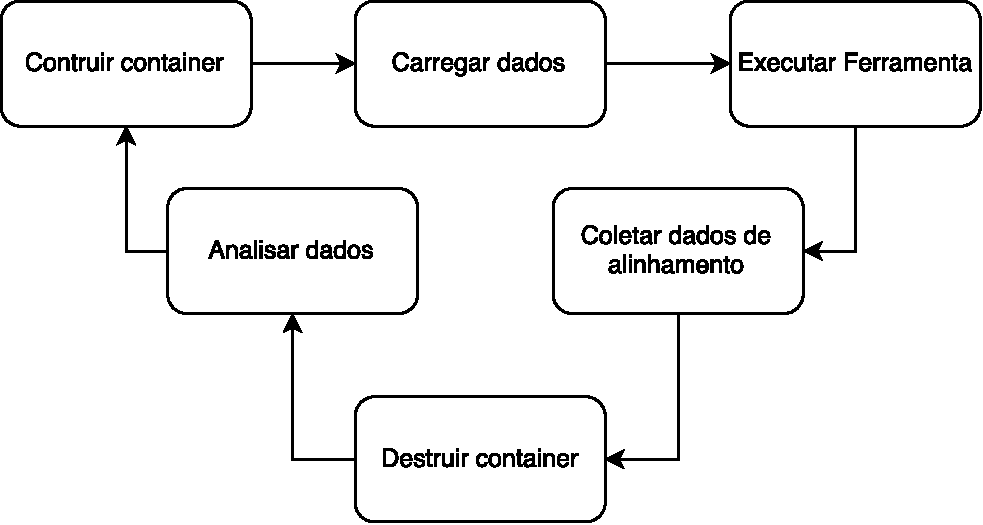
\includegraphics[width=0.9\textwidth]{./imagens/experimento.pdf}
	\caption{Processo de execução do experimento}
	\label{fig:experiment}
\end{figure}

\subsection{Coleta dos Dados}
Os dados utilizados neste estudo foram fornecidos pela OAEI. O \textit{dataset}\footnote{\url{http://islab.di.unimi.it/content/im_oaei/2016/\#doremus}} é composto por três variações (9-heterogeneities,4-heterogeneities e falsepositives-trap). Cada uma das variações conta com um alinhamento de referência, para que seja possível calcular as métricas.

%-----------------------------------------------------------
\section{Execução do experimento}
Para avaliar as ferramentas para correspondência de instância, o experimento irá contar com dois cenários possíveis, com uma execução para cada nível dos fatores definidos na subseção \ref{sub:fator_nivel} , totalizando 6 execuções. A Tabela \ref{tab:cenarios} apresenta os cenários. 

\begin{table}[h]
	\centering
	\caption{Cenários de alinhamento}
	\label{tab:cenarios}
	\begin{tabular}{|c|c|}
		\hline
		\textbf{Cenário} & \textbf{Datasets}          \\ \hline
		C1               & 9-heterogeneities          \\ \hline
		C2               & falsepositives-trap        \\ \hline
	\end{tabular}
\end{table}

\subsection{Instrumentação}
Para a realização do experimento de correspondência de instâncias, serão utilizados os seguintes instrumentos.

\begin{itemize}
\item Intellij IDEA 2016.3 para desenvolvimento do código e execução da proposta.
\item Virtuoso RDF Store - 07.20.3217;
\item OpenJDK 64-Bit Server VM (build 25.111-b14, mixed mode)
\end{itemize}

Para isolar os efeitos entre as execuções, todo o experimento foi conduzido em um contêiner, que permite isolar as aplicações, fazendo com que as aplicações sejam executadas em ambientes idênticos sem que gerem efeitos colaterais entre si.

\subsection{Ameaças à validade}
Embora todo experimento tenha sido projetado para minimizar possíveis ameaças que comprometam suas conclusões, existem algumas ameaças que devem ser mencionadas. Nos tópicos a seguir, serão apresentadas e detalhadas as ameaças deste experimento.

\subsubsection{Ameaças à validade interna}
Uma possível ameaça interna à validade do experimento pode ser a seleção das unidades experimentais, pois os \textit{dataset} utilizados no experimento foram fornecidos pelo OAEI e nenhum outro \textit{dataset} foi utilizado.

\subsubsection{Ameaças à validade externa}
As unidades experimentais desta pesquisa são selecionadas de apenas uma base de dados correspondente a cada modelo, tendo, cada uma delas, características que poderão não ser generalizadas para as demais bases

\subsubsection{Ameaças à validade de construto}
É possível que a quantidade de fatores e cenários não sejam suficientes para observar diferenças significativas na eficácia entre as abordagens utilizadas para a correspondência de instâncias. Além disso, deve-se considerar que o tempo de resposta não foi considerado no experimento.

\subsubsection{Ameaças à validade de conclusão}
Devido a pequena quantidade de dados por \textit{dataset}, é possível que a quantidade de instâncias por \textit{dataset}, não seja suficiente para observar diferenças significativas nas métricas associadas.

\section{Análise dos Resultados}
O experimento foi conduzido de acordo com o planejamento descrito anteriormente neste capítulo, depois da execução, os \textit{datasets} de alinhamento eram coletados. Os dados de precisão, revocação e medida-f eram calculados de acordo com as funções especificadas anteriormente.
Ao longo desta seção, uma análise descritiva dos dados obtidos será conduzida, envolve, a apresentação das métricas referentes a cada cenário.

As figuras \ref{fig:cenario1}, \ref{fig:cenario2} apresentam as ferramentas de acordo com seus resultados em cada um dos cenários. A Tabela \ref{tab:resultados} sumariza os dados obtidos para cada cenário.

\begin{table}[h]
	\centering
	\caption{Sumarização dos dados relativos a precisão, revocação e medida-f por cenário.}
	\label{tab:resultados}
	\begin{tabular}{|c|c|c|c|c|}
		\hline
		      Cenário       & Ferramenta & Precisão & Revocação & Medida-F \\ \hline
		\multirow{3}{*}{C1} &  Proposta  &    1     &   0.875   &  0.933   \\ \cline{2-5}
		                    &    AML     &  0.966   &   0.875   &  0.918   \\ \cline{2-5}
		                    &   RiMOM    &  0.813   &   0.813   &  0.813   \\ \hline
		\multirow{3}{*}{C2} &    AML     &  0.921   &   0.854   &  0.886   \\ \cline{2-5}
		                    &  Proposta  &  0.906   &   0.707   &  0.794   \\ \cline{2-5}
		                    &   RiMOM    &  0.707   &   0.707   &  0.707   \\ \hline
	\end{tabular}
\end{table}

\begin{center}
\begin{figure}
	\begin{tikzpicture}[cap=round]{H}
	%\draw[step=1cm,very thin,color=gray] (0,0) grid (10.0,9.0);
	\draw[|-|] (-0,0) -- (10,0);
	\draw[dashed,very thin] (10,0) arc (0:60:10cm);
	\draw[dashed,very thin] (0,0) arc (180:120:10cm);
	\draw[dashed] (10,0) arc (0:60:10cm) node[anchor=south east]  {{\tiny R=1.}};
	\draw[dashed,very thin] (9,0) arc (0:63:9cm) node[anchor=south east] {{\tiny R=.9}};
	\draw[dashed,very thin] (8,0) arc (0:66:8cm) node[anchor=south east]  {{\tiny R=.8}};
	\draw[dashed,very thin] (7,0) arc (0:70:7cm) node[anchor=south east]  {{\tiny R=.7}};
	\draw[dashed,very thin] (6,0) arc (0:73:6cm) node[anchor=south east]  {{\tiny R=.6}};
	\draw[dashed,very thin] (5,0) arc (0:76:5cm) node[anchor=south east] {{\tiny R=.5}};
	\draw[dashed,very thin] (4,0) arc (0:78:4cm) node[anchor=south east] {{\tiny R=.4}};
	\draw[dashed,very thin] (3,0) arc (0:80:3cm) node[anchor=south east] {{\tiny R=.3}};
	\draw[dashed,very thin] (2,0) arc (0:82:2cm) node[anchor=south east] {{\tiny R=.2}};
	\draw[dashed,very thin] (1,0) arc (0:84:1cm) node[anchor=south east] {{\tiny R=.1}};
	\draw[dashed] (0,0) arc (180:120:10cm) node[anchor=south west] {{\tiny P=1.}};
	\draw[dashed,very thin] (1,0) arc (180:117:9cm) node[anchor=south west] {{\tiny P=.9}};
	\draw[dashed,very thin] (2,0) arc (180:114:8cm) node[anchor=south west] {{\tiny P=.8}};
	\draw[dashed,very thin] (3,0) arc (180:110:7cm) node[anchor=south west] {{\tiny P=.7}};
	\draw[dashed,very thin] (4,0) arc (180:107:6cm) node[anchor=south west] {{\tiny P=.6}};
	\draw[dashed,very thin] (5,0) arc (180:105:5cm) node[anchor=south west] {{\tiny P=.5}};
	\draw[dashed,very thin] (6,0) arc (180:103:4cm) node[anchor=south west] {{\tiny P=.4}};
	\draw[dashed,very thin] (7,0) arc (180:100:3cm) node[anchor=south west] {{\tiny P=.3}};
	\draw[dashed,very thin] (8,0) arc (180:96:2cm) node[anchor=south west] {{\tiny P=.2}};
	\draw[dashed,very thin] (9,0) arc (180:90:1cm) node[anchor=south west] {{\tiny P=.1}};
	\draw (0.56,3.29) node[anchor=south west] {\tiny{F=0.5}};
	\draw plot[smooth] coordinates { (0.56,3.29) (1.55,3.10) (2.46,2.68) (3.31,2.05) (4.12,1.19) (5.00,0.00) (6.42,1.79) (9.44,3.29)};
	\draw (0.92,4.19) node[anchor=south west] {\tiny{F=0.6}};
	\draw plot[smooth] coordinates { (0.92,4.19) (1.96,4.05) (2.95,3.78) (3.93,3.48) (5.00,3.32) (6.56,3.63) (9.08,4.19)};
	\draw (1.45,5.19) node[anchor=south west] {\tiny{F=0.7}};
	\draw plot[smooth] coordinates { (1.45,5.19) (2.59,5.11) (3.74,4.98) (5.00,4.90) (6.73,5.03) (8.55,5.19)};
	\draw (2.22,6.29) node[anchor=south west] {\tiny{F=0.8}};
	\draw plot[smooth] coordinates { (2.22,6.29) (3.54,6.27) (5.00,6.24) (6.91,6.28) (7.78,6.29)};
	\draw (3.35,7.47) node[anchor=south west] {\tiny{F=0.9}};
	\draw plot[smooth] coordinates { (3.35,7.47) (5.00,7.48) (6.65,7.47)};
	\draw (0,-0.6) node {$Revocacao$};
	\draw (10,-0.6) node {$Precisao$};
	%\draw (-0.2,0) node {0}; 
	%\draw (10.2,0) node {1}; 
	\draw plot[mark=*,] coordinates {(6.171875,7.86816109293)};
	\draw (6.181875,7.87816109293) node[anchor=south west] {Proposta};
	\draw plot[mark=*,] coordinates {(5.837655,7.69658262484)};
	\draw (5.847655,7.70658262484) node[anchor=south west] {AML};
	\draw plot[mark=*,] coordinates {(5.0,6.41068639071)};
	\draw (5.01,6.42068639071) node[anchor=south west] {RIMOM};
	\end{tikzpicture}
	\caption{Resultado das ferramentas para o cenário 1}
	\label{fig:cenario1}
\end{figure}
\begin{figure}
		\begin{tikzpicture}[cap=round]{H}
		%\draw[step=1cm,very thin,color=gray] (0,0) grid (10.0,9.0);
		\draw[|-|] (-0,0) -- (10,0);
		\draw[dashed,very thin] (10,0) arc (0:60:10cm);
		\draw[dashed,very thin] (0,0) arc (180:120:10cm);
		\draw[dashed] (10,0) arc (0:60:10cm) node[anchor=south east]  {{\tiny R=1.}};
		\draw[dashed,very thin] (9,0) arc (0:63:9cm) node[anchor=south east] {{\tiny R=.9}};
		\draw[dashed,very thin] (8,0) arc (0:66:8cm) node[anchor=south east]  {{\tiny R=.8}};
		\draw[dashed,very thin] (7,0) arc (0:70:7cm) node[anchor=south east]  {{\tiny R=.7}};
		\draw[dashed,very thin] (6,0) arc (0:73:6cm) node[anchor=south east]  {{\tiny R=.6}};
		\draw[dashed,very thin] (5,0) arc (0:76:5cm) node[anchor=south east] {{\tiny R=.5}};
		\draw[dashed,very thin] (4,0) arc (0:78:4cm) node[anchor=south east] {{\tiny R=.4}};
		\draw[dashed,very thin] (3,0) arc (0:80:3cm) node[anchor=south east] {{\tiny R=.3}};
		\draw[dashed,very thin] (2,0) arc (0:82:2cm) node[anchor=south east] {{\tiny R=.2}};
		\draw[dashed,very thin] (1,0) arc (0:84:1cm) node[anchor=south east] {{\tiny R=.1}};
		\draw[dashed] (0,0) arc (180:120:10cm) node[anchor=south west] {{\tiny P=1.}};
		\draw[dashed,very thin] (1,0) arc (180:117:9cm) node[anchor=south west] {{\tiny P=.9}};
		\draw[dashed,very thin] (2,0) arc (180:114:8cm) node[anchor=south west] {{\tiny P=.8}};
		\draw[dashed,very thin] (3,0) arc (180:110:7cm) node[anchor=south west] {{\tiny P=.7}};
		\draw[dashed,very thin] (4,0) arc (180:107:6cm) node[anchor=south west] {{\tiny P=.6}};
		\draw[dashed,very thin] (5,0) arc (180:105:5cm) node[anchor=south west] {{\tiny P=.5}};
		\draw[dashed,very thin] (6,0) arc (180:103:4cm) node[anchor=south west] {{\tiny P=.4}};
		\draw[dashed,very thin] (7,0) arc (180:100:3cm) node[anchor=south west] {{\tiny P=.3}};
		\draw[dashed,very thin] (8,0) arc (180:96:2cm) node[anchor=south west] {{\tiny P=.2}};
		\draw[dashed,very thin] (9,0) arc (180:90:1cm) node[anchor=south west] {{\tiny P=.1}};
		\draw (0.56,3.29) node[anchor=south west] {\tiny{F=0.5}};
		\draw plot[smooth] coordinates { (0.56,3.29) (1.55,3.10) (2.46,2.68) (3.31,2.05) (4.12,1.19) (5.00,0.00) (6.42,1.79) (9.44,3.29)};
		\draw (0.92,4.19) node[anchor=south west] {\tiny{F=0.6}};
		\draw plot[smooth] coordinates { (0.92,4.19) (1.96,4.05) (2.95,3.78) (3.93,3.48) (5.00,3.32) (6.56,3.63) (9.08,4.19)};
		\draw (1.45,5.19) node[anchor=south west] {\tiny{F=0.7}};
		\draw plot[smooth] coordinates { (1.45,5.19) (2.59,5.11) (3.74,4.98) (5.00,4.90) (6.73,5.03) (8.55,5.19)};
		\draw (2.22,6.29) node[anchor=south west] {\tiny{F=0.8}};
		\draw plot[smooth] coordinates { (2.22,6.29) (3.54,6.27) (5.00,6.24) (6.91,6.28) (7.78,6.29)};
		\draw (3.35,7.47) node[anchor=south west] {\tiny{F=0.9}};
		\draw plot[smooth] coordinates { (3.35,7.47) (5.00,7.48) (6.65,7.47)};
		\draw (0,-0.6) node {$Revocacao$};
		\draw (10,-0.6) node {$Precisao$};
		%\draw (-0.2,0) node {0}; 
		%\draw (10.2,0) node {1}; 
		\draw plot[mark=*,] coordinates {(6.604935,6.20148640616)};
		\draw (6.614935,6.21148640616) node[anchor=south west] {Proposta};
		\draw plot[mark=*,] coordinates {(5.0,4.99848977192)};
		\draw (5.01,5.00848977192) node[anchor=south west] {RiMOM};
		\draw plot[mark=*,] coordinates {(5.594625,7.31602836991)};
		\draw (5.604625,7.32602836991) node[anchor=south west] {AML};
		\end{tikzpicture}
		\caption{Resultado das ferramentas para o cenário 2}
		\label{fig:cenario2}
\end{figure}
\end{center}

\subsection{Verificação das hipóteses}
Esta seção tem como objetivo validar ou refutar as hipóteses propostas. A primeira hipótese a ser verificada será feita com relação à precisão. As hipóteses nula e alternativa estão numeradas abaixo, respectivamente:
on
\begin{itemize}
\item \textbf{H1-0:} A precisão apresentada pelas abordagens é igual.
\item \textbf{H1-1:} A precisão apresentada pelas abordagens é diferente.
\end{itemize}

Para realizar a análise, devemos observar a precisão nos dois cenários de alinhamento. Como descrito na Tabela \ref{tab:resultados}, a proposta apresentou precisão de 1 para o cenário 1 e 0.906 para o cenário 2, refutando a hipótese nula (H1-0).

A próxima validação de hipótese ocorrerá com relação à revocação. As hipóteses nula e alternativa estão numeradas abaixo, respectivamente:

\begin{itemize}
\item \textbf{H2-0:} A revocação apresentada pelas abordagens é igual.
\item \textbf{H2-1:} A revocação apresentada pelas abordagens é diferente.
\end{itemize}

Diante do resultado apresentado pelas ferramentas nos dois cenários de alinhamento, onde apresentou uma revocação de 0.875 para o cenário 1 e 0.707 para o cenário 2. Apesar do bom desempenho, a proposta apresentou valores iguais a pelo menos uma das ferramentas em cada um dos cenários. Dessa forma, não é possível refutar a hipótese nula (H2-0).

Finalizando a verificação de hipóteses, serão analisadas as hipóteses relacionadas à medida-f.As hipóteses nula e alternativa estão numeradas abaixo, respectivamente:

\begin{itemize}
\item \textbf{H3-0:} A medida-f apresentada pelas abordagens é igual.
\item \textbf{H3-1:} A medida-f apresentada pelas abordagens é diferente.
\end{itemize}

Conforme os resultados apresentados na Tabela \ref{tab:resultados}, a proposta ficou em primeiro posição no cenário 1 com uma dedida-f de 0.933 e segundo lugar no cenário 2 com 0.794.

\section{Principais conclusões}
O experimento conduzido neste capítulo, visou avaliar a eficácia das ferramentas de alinhamento de dados conectados com relação às métricas de precisão, revocação e medida-f. Essas variáveis foram avaliadas separadamente em cada um dos dois cenários de alinhamento (9-heterogeneities e falsepositives-trap).

Pelas análises realizadas, foi possível verificar que a proposta apresentou bons resultados mesmo não utilizando abordagens dedicadas ao \textit{dataset}.
\chapter{Estudo de caso (QIE)}
\label{cap:estudo}
Neste capítulo será descrita a utilização do processo de alinhamento através de um estudo de caso, o QIE. O QIE foi escolhido, pois se trata de um projeto que pretende cruzar informações sobre a comunidade brasileira de informática na educação. Este capítulo está estruturado em três seções. A seção \ref{sec:estudo_descricao} apresenta uma descrição do estudo de caso e a conversão dos dados para RDF.

\section{Descrição do estudo}
\label{sec:estudo_descricao}
Para validar a eficácia da solução, foi solicitado a membros da comunidade de informática na educação que sugerissem perguntas de seu interesse. Como resultado foi levantado um conjunto contendo mais de 30 questões. A Tabela \ref{tab:questions} apresenta as questões propostas pelos membros.

\begin{table}[!ht]
	\centering
	\caption{Perguntas sugeridas pela comunidade}
	\label{tab:questions}
	\begin{tabular}{|l|l|}
		\hline
		ID  & Questões                                                                          \\ \hline
		Q01 & Quantos pesquisadores?                                                            \\ \hline
		Q02 & Quais pesquisadores?                                                              \\ \hline
		Q03 & Onde estão? (Estado)                                                              \\ \hline
		Q04 & Onde estão? (Universidade)                                                        \\ \hline
		Q05 & Quais são Doutores?                                                               \\ \hline
		Q06 & Quantos são Doutores?                                                             \\ \hline
		Q07 & Quem possui marca?                                                                \\ \hline
		Q08 & Onde fizemos os nossos doutorados?                                                \\ \hline
		Q09 & Onde fizemos os nossos pós-doutorados?                                            \\ \hline
		Q10 & Quantas publicações o autor “z” tem no evento “x”?                                \\ \hline
		Q11 & Quantos trabalhos foram publicados no evento “x”?                                 \\ \hline
		Q12 & Quantos autores publicaram no evento “x”?                                         \\ \hline
		Q13 & Quantos artigos foram publicados no periódico “y”?                                \\ \hline
		Q14 & Lista de Doutores + Email (RBIE)                                                  \\ \hline
		Q15 & Lista de Autores + Competência + Email                                            \\ \hline
		Q16 & Lista de Artigos publicados na RBIE - Geral                                       \\ \hline
		Q17 & Quantos são bolsistas e qual o nível? (DT/PQ)                                     \\ \hline
		Q18 & Quais são as principais competências da comunidade de IE?                         \\ \hline
		Q19 & Quais conceitos são explorados?                                                   \\ \hline
		Q20 & Quais os temas são mais pesquisados em IE?                                        \\ \hline
		Q21 & Quais pesquisadores colaboram entre si?                                           \\ \hline
		Q22 & Quais instituições colaboram entre si?                                            \\ \hline
		Q23 & Quais são os trabalhos relacionados?                                              \\ \hline
		Q24 & Como os conceitos explorados evoluem ao longo do tempo?                           \\ \hline
		Q25 & Mapa de tendências de pesquisa em uma linha do tempo.                             \\ \hline
		Q26 & O quão um pesquisador X está publicando no SBIE, WIE e RBIE ao longo do tempo?    \\ \hline
		Q27 & Lista de bolsistas de produtividade                                               \\ \hline
		Q28 & Quais as instituições?                                                            \\ \hline
		Q29 & Quais autores publicaram na conferência "X"?                                      \\ \hline
		Q30 & Quantos pesquisadores de IE estão em PPGs de CC?                                  \\ \hline
		Q31 & Quem são os maiores especialistas em recursos digitais e objetos de aprendizagem? \\ \hline
	\end{tabular}
\end{table}

De acordo com as perguntas realizadas, pode-se perceber que em alguns momentos é necessário o cruzamento de informações dos pesquisadores e suas publicações de diferentes fontes. , sendo elas a Revista Brasileira de Informática na Educação\footnote{\url{http://www.br-ie.org/pub/index.php/rbie}} (RBIE), Workshop de informática na Escola\footnote{\url{http://www.br-ie.org/pub/index.php/wie }} (WIE), Simpósio Brasileiro de Informática na Educação\footnote{\url{http://www.br-ie.org/pub/index.php/sbie}} (SBIE) e currículum Lattes\footnote{\url{http://lattes.cnpq.br}}. Vale a pena ressaltar que os \textit{datasets} foram disponibilizados como arquivos XML, sendo necessário transformá-los para RDF.

Para modelar os dados, foram utilizadas as ontologias dac\footnote{\url{https://github.com/josmarios/dac/blob/master/Ontologies/dacV2.1.owl}} e lattes\footnote{\url{https://github.com/armandobs14/lattes/blob/master/lattes.owl}}. A primeira tem o objetivo de modelar o domínio de publicação (ver Figura \ref{fig:dac}). A segunda foi construída para modelar o domínio do lattes (ver Figura \ref{fig:lattes}).

\begin{figure}[!ht]
	\centering
	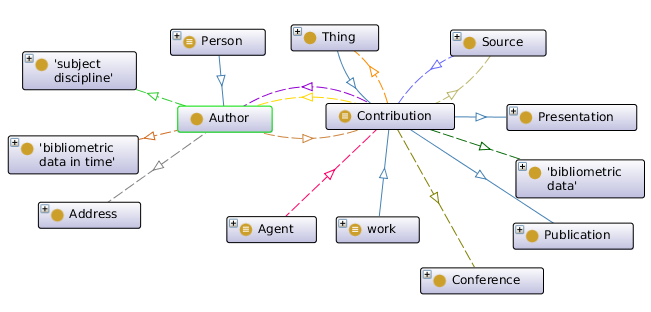
\includegraphics[width=0.9\textwidth]{./imagens/dac-mainview.png}
	\caption{Taxonomia da ontologia dac}
	\label{fig:dac}
\end{figure}

\begin{figure}[!ht]
	\centering
	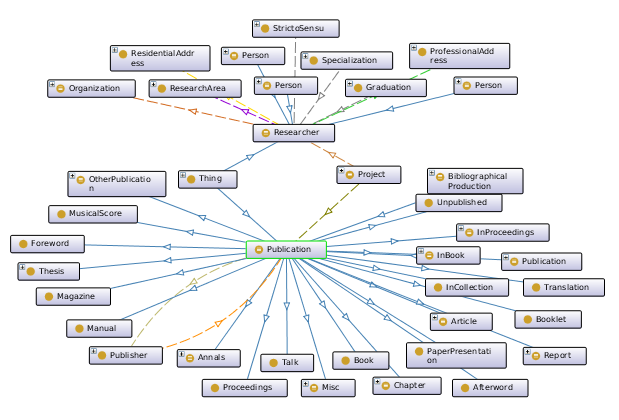
\includegraphics[width=0.9\textwidth]{./imagens/lattes-mainview.png}
	\caption{Taxonomia da ontologia lattes}
	\label{fig:lattes}
\end{figure}

Para transformar os dados para RDF foi utilizada a ferramenta OpenRefine\footnote{\url{http://openrefine.org}} com a extensão para suportar RDF. Essa ferramenta foi selecionada devido a sua facilidade para criar os templates de transformação. Após a transformação dos dados, as ontologias e os dados foram persistidos no Virtuoso\footnote{\url{https://virtuoso.openlinksw.com}}. A Figura \ref{fig:conversao} representa o processo de conversão dos dados.

\begin{figure}[!ht]
	\centering
	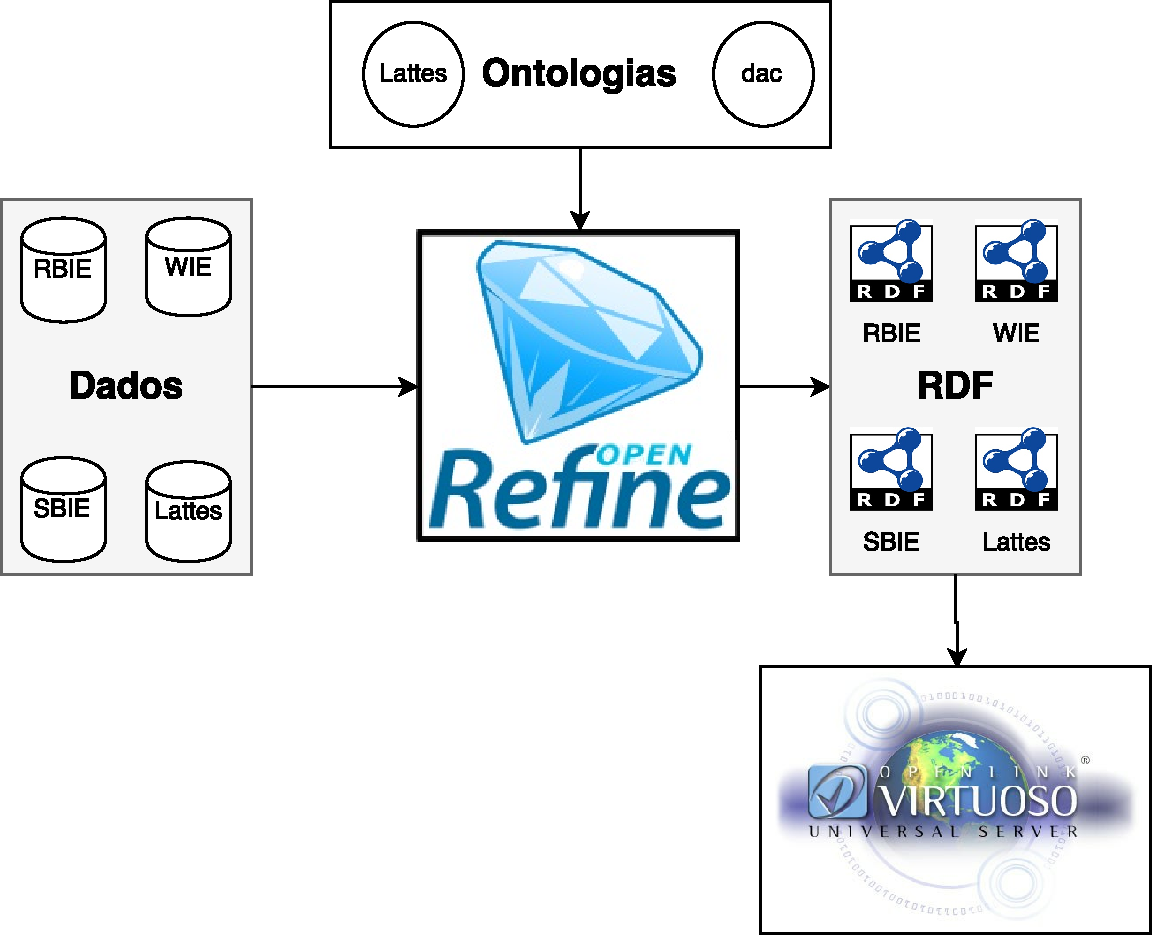
\includegraphics[width=0.8\textwidth]{./imagens/conversao.pdf}
	\caption{Processo de conversão para rdf}
	\label{fig:conversao}
\end{figure}

Com o processo de conversão dos dados foram geradas 1,1 Milhão de triplas, sendo distribuídas da seguinte forma: (96\%, 1.094.307 triplas) pertencem ao Lattes, (1,61\%; 18.363 triplas) pertencem ao SBIE, (1,21\%; 14.601 triplas) pertencem ao WIE e (1,1\%; 12.503 triplas) pertencem ao RBIE.

\newpage
\section{Execução do processo}
Nesta seção pretende-se descrever como foi realizada cada uma das etapas do processo de correspondência. 

\subsection{Selecionar \textit{Datasets}}
\label{sub:selecionar_datasets}
Esta etapa diz respeito a seleção de quais \textit{datasets} serão utilizados como entrada para o processo de correspondência de instâncias. Vale ressaltar que dois ou mais \textit{datasets} podem ser selecionados. Neste contexto, foram selecionados os \textit{datasets} do RBIE, SBIE, WIE e Lattes.
  
\subsection{Identificar Conceitos}
Esta etapa do processo diz respeito a seleção dos conceitos (principal e relacionados), que serão utilizados no processo. Atualmente existem apenas uma restrição quanto a seleção dos conceitos, neste é possível selecionar apenas um conceito principal.

\subsubsection{Conceito Principal}
Como descrito na seção \ref{sec:prop_identificar} para facilitar a identificação do conceito principal por parte do usuário a consulta \ref{lst:sparql} foi desenvolvida. A Tabela \ref{tab:estudo_sparql1} apresenta os resultados obtidos através execução da consulta. 

\begin{table}[h]
	\centering
	\caption{Conceito da ontologia e quantidade de instâncias}
	\label{tab:estudo_sparql1}
	\begin{tabular}{@{}|l|r|@{}}
		\hline
		\multicolumn{1}{|c|}{\textbf{Conceitos}}               & \multicolumn{1}{c|}{\textbf{quantidade}} \\ \hline
		http://www.ic.ufal.br/dac/Contribution               & 868752                              \\ \hline
		http://www.ic.ufal.br/dac/Author                     & 155680                              \\ \hline
		http://www.ic.ufal.br/lattes/DoctoralDegree          & 2387                                \\ \hline
		http://www.ic.ufal.br/lattes/Graduation              & 2195                                \\ \hline
		http://www.w3.org/2002/07/owl\#Class                 & 1680                                \\ \hline
		http://www.ic.ufal.br/lattes/Course                  & 1186                                \\ \hline
		http://www.w3.org/1999/02/22-rdf-syntax-ns\#List     & 204                                 \\ \hline
		http://www.w3.org/2002/07/owl\#Restriction           & 161                                 \\ \hline
		http://www.w3.org/2002/07/owl\#ObjectProperty        & 128                                 \\ \hline
		http://www.w3.org/2000/01/rdf-schema\#Class          & 60                                  \\ \hline
		http://www.w3.org/2002/07/owl\#Ontology              & 24                                  \\ \hline
		http://www.w3.org/1999/02/22-rdf-syntax-ns\#Property & 23                                  \\ \hline
		http://purl.org/dc/terms/AgentClass                  & 3                                   \\ \hline
	\end{tabular}
\end{table}

Apesar de ter a segunda maior quantidade de instância nos dados, o conceito \textbf{\textit{Author}} foi selecionado como conceito principal. A escolhe desse conceito deu-se não só pela quantidade de instâncias, mas também por questões estratégicas, visto que a proposta deste estudo de caso é cruzar informações de pesquisadores.

\subsubsection{Conceito Relacionado}
Para selecionar o conceito relacionado que será utilizado, foi executada a consulta \ref{lst:sparql2}. A tabela \ref{tab:estudo_sparql2} apresenta os conceitos relacionados ao conceito principal previamente selecionado.

\begin{table}[h]
	\centering
	\caption{Lista com conceitos relacionados}
	\label{tab:estudo_sparql2}
	\begin{tabular}{@{}|l|@{}}
		\hline
		\multicolumn{1}{|c|}{\textbf{Conceito Relacionado}}        \\ \hline
		http://www.ic.ufal.br/dac/Contribution                     \\ \hline
		http://www.ic.ufal.br/lattes/Software                      \\ \hline
		http://www.ic.ufal.br/lattes/TradeMark                     \\ \hline
		http://xmlns.com/foaf/0.1/Organization                     \\ \hline
		http://www.ic.ufal.br/lattes/Organization                  \\ \hline
		http://www.nees.com.br/boa-moradia/crawler/LocalityAddress \\ \hline
		http://www.ic.ufal.br/lattes/DoctoralDegree                \\ \hline
		http://www.ic.ufal.br/lattes/Graduation                    \\ \hline
		http://www.ic.ufal.br/lattes/MastersDegree                 \\ \hline
	\end{tabular}
\end{table}
 
O conceito \textbf{\textit{Contribution}} foi selecionado como conceito relacionado. Esse conceito será utilizado durante o alinhamento em cascata. Vale ressaltar que mais de um conceito relacionado pode ser selecionado.
 
\subsection{Listar Recursos}
A lista de recursos é gerada de forma automática com base nos conceitos selecionados anteriormente. A partir da lista de recursos serão montados os pares candidatos. Vale ressaltar que no estudo em questão um \textit{dataset} pode conter mais de uma instância para a mesma entidade do mundo real (e.g. mais de uma URI para o mesmo pesquisador). Dessa forma, foram gerados pares candidatos dentro do mesmo \textit{dataset}, caracterizando o alinhamento interno.

\subsection{Alinhar Dados}
A etapa de alinhamento é responsável por determinar se um par candidato diz respeito à mesma entidade do mundo real. Neste processo existem duas abordagens de alinhamento sendo elas simples e em cascata. Na abordagem simples, os recursos são comparados diretamente, explorando as propriedades e suas características. Na abordagem em cascata os recursos são comparados a partir dos recursos relacionados.

\subsubsection{Alinhamento Simples}
Assim como outras abordagens para a correspondência de instâncias \cite{zhang2016rimom}, também foi utilizado funções que analisam a similaridade entre dois recursos. Para determinar a similaridade entre os pares foi utilizado a função \ref{eq:similaridade}. Essa função de similaridade gera valores entre 0 e 1, sendo 0 totalmente distintos e 1 iguais. Além da função utilizada, foram definidos limiares (\textit{threshold}). Isso quer dizer que valores de similaridade acima do limiar eram considerados correspondentes. 
Inicialmente o valor do limiar foi definido de forma arbitrária e posteriormente ajustado com ajuda de testes. Nesses testes eram avaliados vários limiares com o objetivo de escolher o de melhor custo/benefício. Por fim, o valor do limiar foi estabelecido em 0.88.


\subsubsection{Alinhamento em Cascata}
O alinhamento em cascata consiste em alinhar instâncias do recurso principal a partir de recursos relacionados. Esta etapa do processo é executada para cada um dos conceitos relacionados selecionados na etapa de identificação de conceitos e consiste de três atividades:
\begin{itemize}
	\item \textbf{Alinhar dos recursos relacionados:} O alinhamento simples é executado entre as instâncias que pertencem ao conceito relacionado;
	
	\item \textbf{Recuperar instâncias do conceito principal:} A partir do alinhamento entre instâncias de recurso relacionado, as instâncias que pertencem ao conceito principal são recuperadas.
	
	\item \textbf{Alinhar instâncias do conceito principal:} A partir das instâncias recuperadas novos pares candidatos são gerados e passados como entrada para o alinhamento simples.
\end{itemize}


\section{Resultados}
Os resultados apresentados nessa seção estão separados em duas partes. A primeira diz respeito aos alinhamentos gerados. A segunda aborda as respostas das perguntas realizadas pela comunidade.

\subsection{Alinhamentos}
Após a realização do alinhamento por parte da ferramenta, foi realizado um levantamento. A partir do levantamento foi possível gerar informações como a quantidade de recursos são repetidos nas bases, total de recursos alinhados com o perfil Lattes, bem como precisão, revocação e medida-f \cite{goutte2005probabilistic} para analisar a confiabilidade dos alinhamentos (ver Tabela \ref{tab:case_study}).

%\begin{landscape}
\begin{table}[!ht]
	\centering
	\caption{ Resultado dos alinhamentos com relação aos dados do Lattes}
	\label{tab:case_study}
	%\begin{tabular}{|p{1cm}|p{2cm}|p{2cm}|p{1cm}|p{1cm}|p{2cm}|p{2cm}|p{2cm}|}
	\begin{tabular}{|c|c|c|c|}
		\hline
		\textbf{Dataset}	&	\textbf{RBIE}	&	\textbf{SBIE}	&	\textbf{WIE}  \\ \hline
		\textbf{Iniciais}	&	1118	&	1687	&	1952 \\ \hline
		%\textbf{Alinhamentos}	&	276	&	1742	&	1637  \\ \hline
		%\textbf{Recursos Alinhados}	&	1029	&	141	&	1405 \\ \hline
		\textbf{Finais}	&	806	&	1032	&	1098 \\ \hline
		\textbf{Perfis com Lattes*}	&	92.03\% (1029)	&	71.54\% (1207)	&	75.20\% (1468) \\ \hline
		\textbf{Perfis com Lattes**}	&	89.06\% (717)	&	70.16\% (792)	&	67.48\% (741) \\ \hline
		\textbf{P | R | F}	&	0.97 | 1 | 0.98	&	0.94 | 1 | 0.97 	&	0.84 | 1 | 0.91 \\ \hline
	\end{tabular}
\end{table}
* - com repetição
** - sem repetição
%\end{landscape}

\subsection{Respostas}
O processo de correspondência de instância permite não só identificar as instâncias que dizem respeito a mesma entidade, mas também permite que informações complementares sejam integradas. Dessa forma, foi necessário consultar mais de uma base ao mesmo tempo para responder as perguntas feitas pela comunidade. Devido a quantidade de perguntas feitas, apenas algumas elas serão apresentadas a seguir. As outras estão disponíveis no Anexo ____.

\subsubsection{Q03 - Onde estão? (Estado)}
Para responder esta pergunta é necessário identificar o perfil dos pesquisadores é necessário cruzar as bases (RBIE, SBIE, WIE e Lattes), pois o endereço profissional está no dataset do lattes



\chapter{Considerações finais e trabalhos futuros}

O trabalho apresentou uma abordagem semiautomática para alinhar \textit{datasets} reais. Através de diagramas de atividades e de componentes foi descrito o processo utilizado para conectar recursos de diferentes \textit{datasets}. Essa proposta se faz necessária justamente pela necessidade de soluções capazes de alinhar dados de forma confiável e com menor conhecimento possível do domínio. Além disso, a solução permite que o alinhamento seja executado diretamente dentro do armazenamento de triplas, não havendo a necessidade de gerar arquivos para alinhar. 

Visando avaliar a abordagem proposta em um cenário real, um estudo de caso foi desenvolvido. Neste estudo, a proposta foi utilizada para alinhar \textit{datasets} do RBIE, SBIE, WIE e Lattes. A utilização da solução de alinhamento permitiu que diversas perguntas pudessem ser respondidas. Além disso, foi possível problemas de erros e insistências nos dados puderam ser encontrados.

Por fim, um experimento foi conduzido  a fim de avaliar e comparar em termos de eficácia através das métricas de precisão, revocação e medida-f. Essas métricas foram avaliadas em dois cenários de alinhamento. O experimento apresentou resultados preliminares satisfatórios com base no desempenho dos trabalhos relacionados, pois em todos os cenários a proposta foi capaz de identificar um número significativo de trabalhos que poderiam ser alinhados. 

\section{Principais contribuições}
As principais contribuições deste trabalho são apresentadas a seguir:
\begin{itemize}
\item Desenvolvimento de processo alinhamento de dados conectados, permitindo que \textit{datasets} reais pudessem ser conectados;
\item Abordagem capaz de calcular a similaridade entre recursos levando em consideração o modelo ontológico;
\item Viabilização da execução do alinhamento diretamente dentro do armazenamento de triplas.
\item  Criação de experimento e estudo de caso para avaliar a eficácia das soluções de alinhamento no estado da arte.
\end{itemize}

\subsection{Limitações e trabalhos futuros}

Algumas questões que não foram foco deste trabalho, mas que devem ser consideradas em trabalhos futuros, são estudos em como a qualidade e o tamanho (quantidade de triplas) do \textit{dataset} impacta na qualidade dos alinhamentos.

Outra questão que não está dentro do escopo deste trabalho, mas que também deve ser levado em consideração, é o alinhamento entre ontologias, pois este trabalho foi desenvolvido com objetivo de alinhar dados. Por tanto, se faz necessário estudar mecanismos que unifiquem soluções para alinhar dados e alinhar ontologias.

Como trabalhos futuros, pretende-se realizar mais experimentos para analisar a eficácia da ferramenta com \textit{datasets} com diversas características (Domínio, quantidade de triplas, qualidade etc.). Além disso, pretende-se disponibilizar a solução como uma infraestrutura de alinhamento disponível na Web, dando acesso aos alinhamentos realizados através da solução. Por fim, outras pesquisas serão aplicadas buscando automatizar ainda mais o processo de alinhamento, mais especificamente a escolha dos conceitos buscando otimizar o desempenho e a qualidade nos alinhamentos obtidos.


% ----------------------------------------------------------
% ELEMENTOS PÓS-TEXTUAIS (Referências, Glossário, Apêndices)
% ----------------------------------------------------------
\postextual

\bibliography{bibliografia}

\end{document}
